\subsection{Toy problem}

To verify the proposed methodological pipeline, an adapted version of the toy problem introduced by \citet{pires_reliability_2024} is adopted in this section and defined by Equation \eqref{eq:toy_problem_equation}. In this formulation, \textbf{R} and \textbf{S} denote the structural resistance and the load demand, respectively. The limit-state function $g(\cdot)$ is defined to explicitly account for time-dependent degradation and modeling uncertainties within a probabilistic framework.

Time dependency is introduced through a linear degradation factor applied to the resistance variable, represented by the function $k_{\text{factor}}(t)$. This factor models a progressive reduction in resistance capacity over the service life, assuming $k_{\text{initial}} = 1.0$ at the initial time and $k_{\text{final}} = 0.3$ at the end of the considered lifetime, $T_f = 100$ years, as expressed in Equation \eqref{eq:k_factor_linear}. Although simplified, this formulation captures the essential effects of long-term deterioration processes commonly considered in structural reliability analyses.

Modeling uncertainties are incorporated through the latent variables $\textbf{Z}_1$ and $\textbf{Z}_2$, which affect the resistance and load terms, respectively. These latent variables are modeled as random variables, introducing additional variability into the realizations of \textbf{R} and \textbf{S} and allowing the uncertainty propagation to be explicitly represented in the limit-state function.

The complete formulation of the adopted limit-state function is presented in Equation \eqref{eq:toy_problem_equation}. The probabilistic characterization of all random variables involved in the model, including their probability distributions and statistical parameters, is summarized in Table~\ref{tab:random_variables_parameters}. Normal distributions are assumed for the resistance and load variables, while lognormal distributions are adopted for the model uncertainty factors, following standard practice in structural reliability modeling.

\begin{equation}
k_{\text{factor}}(t) = 
\begin{cases} 
k_{\text{initial}}, & t \leq 0 \\[5pt]
k_{\text{final}}, & t \geq T_f \\[5pt]
k_{\text{initial}} + (k_{\text{final}} - k_{\text{initial}}) \cdot \dfrac{t}{T_f}, & 0 < t < T_f 
\end{cases}
\label{eq:k_factor_linear}
\end{equation}

\begin{equation}
g(\textbf{R}, \textbf{S}, t) = k_{\text{factor}}(t) \cdot \frac{\textbf{R}}{\textbf{Z}_1} - \textbf{S} \cdot \textbf{Z}_2
\label{eq:toy_problem_equation}
\end{equation}

\begin{table}[H]
\centering
\caption{Statistical parameters and probability distributions of the variables used in the model}
\label{tab:random_variables_parameters}
\begin{tabular}{l c c c c}
\hline
\textbf{Variable} & \textbf{Symbol} & \textbf{Distribution} & \textbf{Mean} & \textbf{Standard Deviation} \\
\hline
Resistance      & $R$     & Normal      & 5.00 & 0.80  \\
Load realization            & $S$     & Normal      & 2.00 & 0.60  \\
Model uncertainty for resistance  & $Z_1$   & Lognormal  & 1.00 & 0.028 \\
Model uncertainty for load & $Z_2$   & Lognormal  & 1.00 & 0.096 \\
\hline
\end{tabular}
\end{table}

The time-dependent analysis is performed considering 10 equally spaced time steps over a 100-year horizon. At each time step, realizations of the limit-state function $g$ are evaluated, enabling the assessment of its temporal evolution. In parallel, the corresponding values of the four GLAM parameters, $\lambda_1$ to $\lambda_4$, are computed and analyzed.

For illustrative purposes, fixed realizations of the resistance and load variables, $r = 5.09$ and $s = 1.80$, are considered together with 2000 samples of the latent variables at each time step. The resulting dataset is depicted in Figure~\ref{fig:g_function_realizations}. Figure~\ref{fig:g_function_realizations}(a) shows the evolution of the limit-state function over time, clearly reflecting the influence of the degradation factor applied to the resistance. Figure~\ref{fig:g_function_realizations}(b) presents the temporal evolution of the GLAM parameters, highlighting distinct trends among $\lambda_1$--$\lambda_4$.
\begin{figure}[H]
    \centering

    \begin{subfigure}{0.9\textwidth}
        \centering
        
\includegraphics[width=\textwidth]{z_time-lapse_g_analysis_en.png}
        \caption{}
        \label{fig:indoor_profiles}
    \end{subfigure}

    \vspace{0.5cm} % espaço vertical entre as figuras

    \begin{subfigure}{0.95\textwidth}
        \centering
        
\includegraphics[width=\textwidth]{z_lambdas_for_r_s_realization_en.png}
        \caption{}
        \label{fig:outdoor_profiles}
    \end{subfigure}

    \caption{Evaluation of the function $g$ over time points. 
    (a) Realizations with fixed values $r = 5.09$ and $s = 1.80$. 
    (b) $\lambda_1$--$\lambda_4$ over the time.}
    \label{fig:g_function_realizations}
\end{figure}

%Antes de realizar o treinamento, foi realizada a analise do comportamento dos lambdas ao longo tempo, poi foi percebida uma baixa variação dos valores de lamba 3 e 4, o que corrobora com a hipotese de não ser necessário treinar esses valores, apenas realizar uma média entre eles. Foi analisado então 1000 amostras e 2000 variáveis latentes para os tempos de 0 e 50 anos. To assess the variability of the GLAM parameters ($\lambda_1$--$\lambda_4$) with respect to Equation \eqref{eq:toy_problem_equation}, we analyze their behavior at time points $t=0$ and $t=50$. Figure \ref{fig:toy_lambda_scatter_grid} presents the scatter plots of 1000 realizations of the random variables $r$ and $s$ for each scenario.

Prior to the training of the surrogate model, an exploratory assessment of the temporal behavior of the GLAM parameters is conducted. This analysis indicates that $\lambda_3$ and $\lambda_4$ exhibit limited variability over time when compared to $\lambda_1$ and $\lambda_2$. Such behavior suggests a reduced sensitivity of $\lambda_3$ and $\lambda_4$ to both the input variables and the degradation process, indicating that their explicit training may not be necessary.

To further support this observation, 1000 realizations of the random variables $r$ and $s$, combined with 2000 samples of the latent variables, are analyzed at $t = 0$ and $t = 50$ years. The corresponding scatter plots are shown in Figure~\ref{fig:toy_lambda_scatter_grid}. The results demonstrate that $\lambda_1$ and $\lambda_2$ present pronounced sensitivity to variations in \textbf{R} and \textbf{S}, whereas $\lambda_3$ and $\lambda_4$ display low dispersion and weak dependence on the input variables.

\begin{figure}[H]
    \centering

    % --- LINHA 1 (Tempo t=0) ---
    \begin{subfigure}[b]{0.24\textwidth}
        \centering
        
\includegraphics[
            width=\textwidth,
            height=0.667\textwidth,
            keepaspectratio
        ]{z_lambda_1_t-0.png}
        \caption{$\lambda_1$ ($t=0$)}
    \end{subfigure}
    \hfill
    \begin{subfigure}[b]{0.24\textwidth}
        \centering
        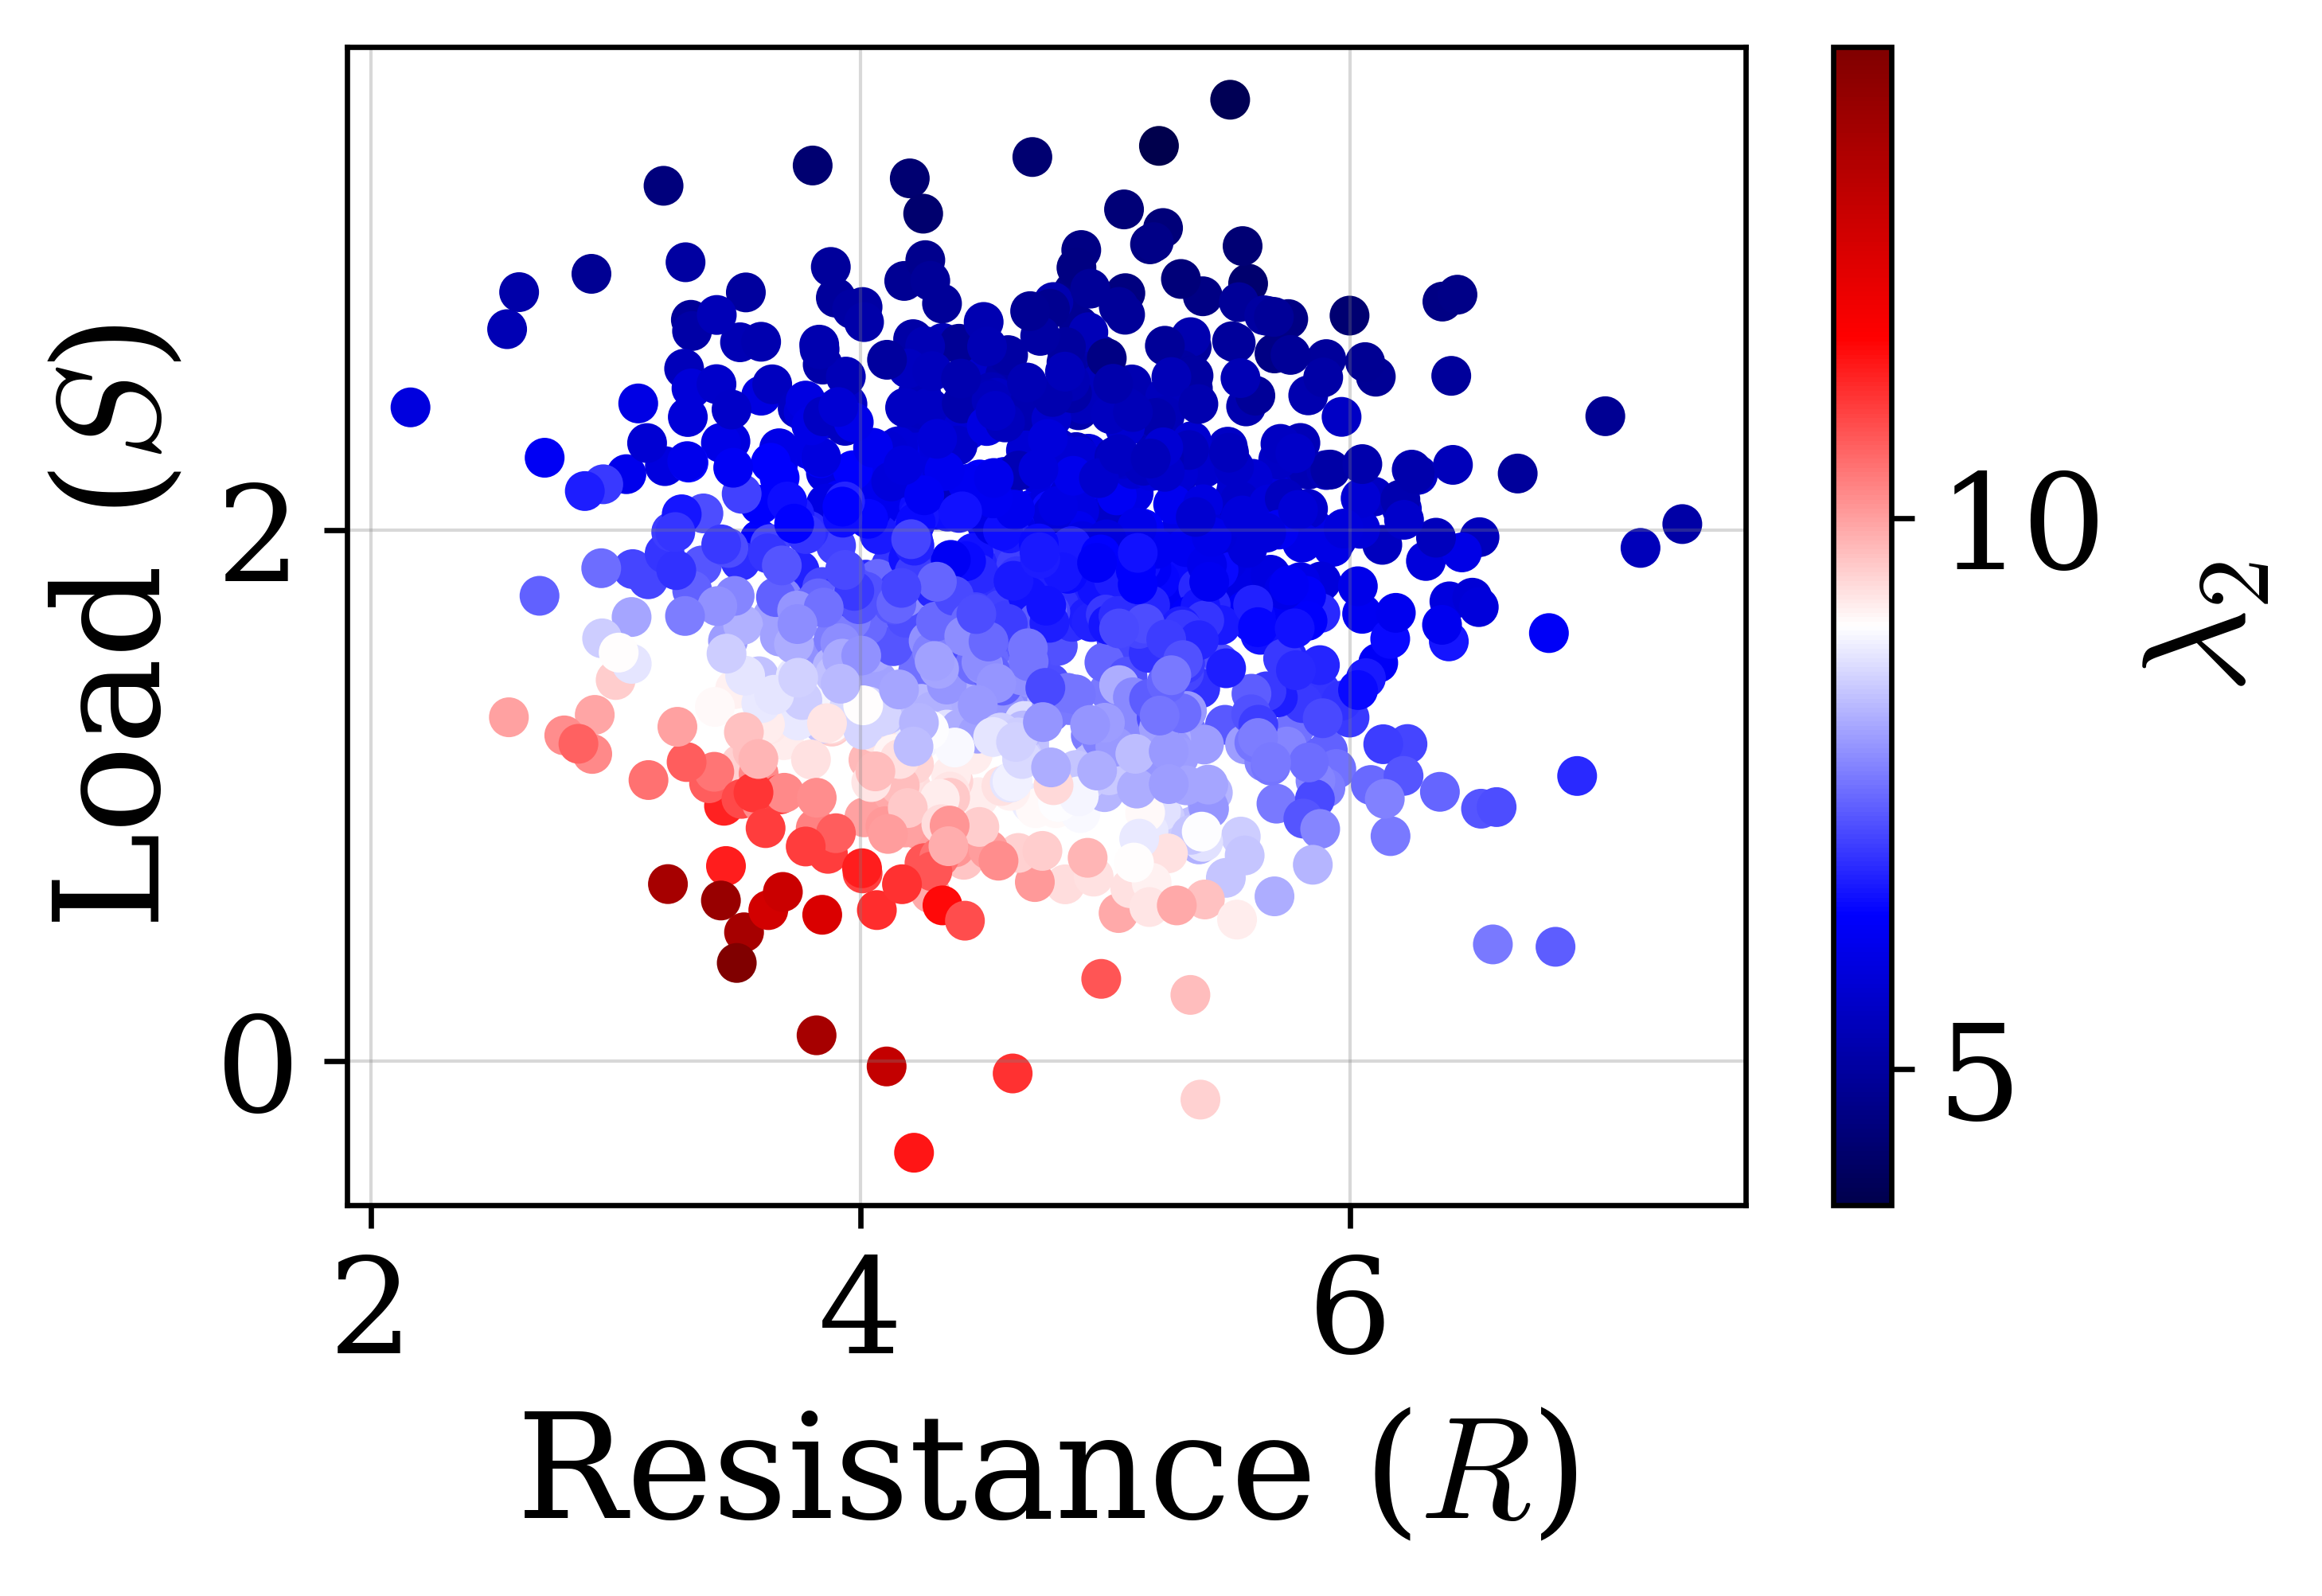
\includegraphics[
            width=\textwidth,
            height=0.667\textwidth,
            keepaspectratio
        ]{z_lambda_2_t-0.png}
        \caption{$\lambda_2$ ($t=0$)}
    \end{subfigure}
    \hfill
    \begin{subfigure}[b]{0.24\textwidth}
        \centering
        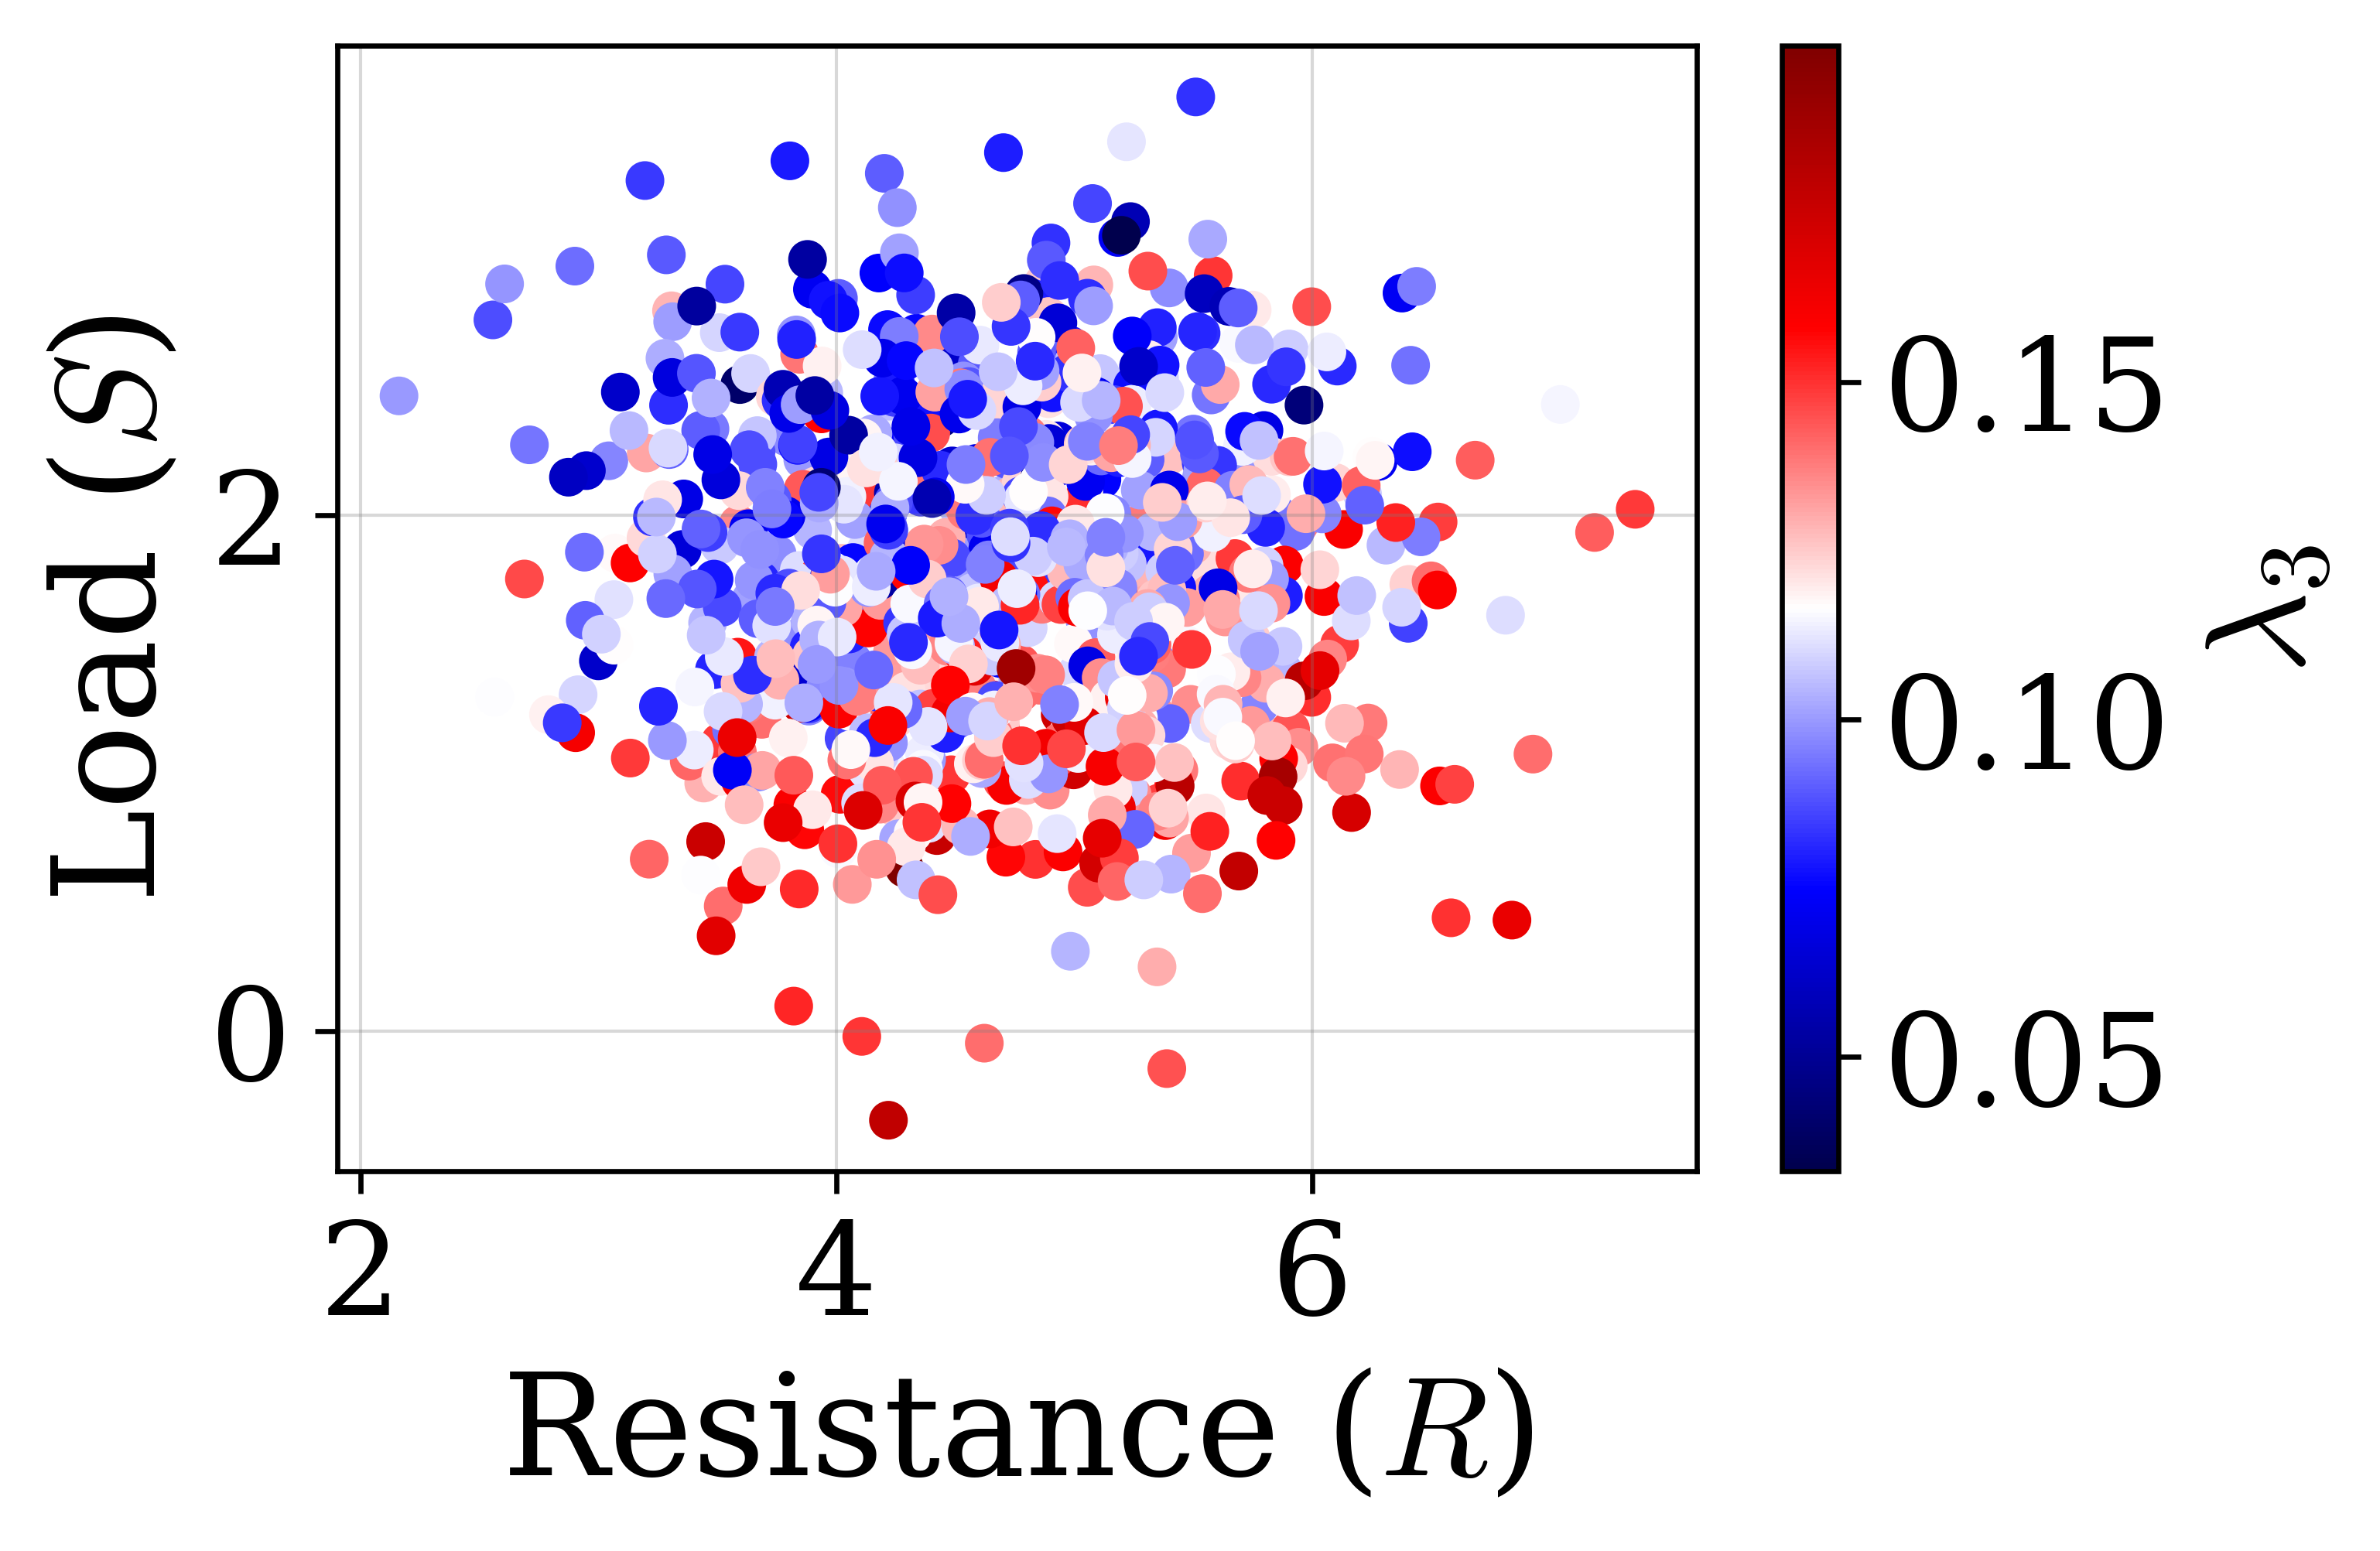
\includegraphics[
            width=\textwidth,
            height=0.667\textwidth,
            keepaspectratio
        ]{z_lambda_3_t-0.png}
        \caption{$\lambda_3$ ($t=0$)}
    \end{subfigure}
    \hfill
    \begin{subfigure}[b]{0.24\textwidth}
        \centering
        
\includegraphics[
            width=\textwidth,
            height=0.667\textwidth,
            keepaspectratio
        ]{z_lambda_4_t-0.png}
        \caption{$\lambda_4$ ($t=0$)}
    \end{subfigure}

    \par\bigskip

    % --- LINHA 2 (Tempo t=50) ---
    \begin{subfigure}[b]{0.24\textwidth}
        \centering
        
\includegraphics[
            width=\textwidth,
            height=0.667\textwidth,
            keepaspectratio
        ]{z_lambda_1_t-50.png}
        \caption{$\lambda_1$ ($t=50$)}
    \end{subfigure}
    \hfill
    \begin{subfigure}[b]{0.24\textwidth}
        \centering
        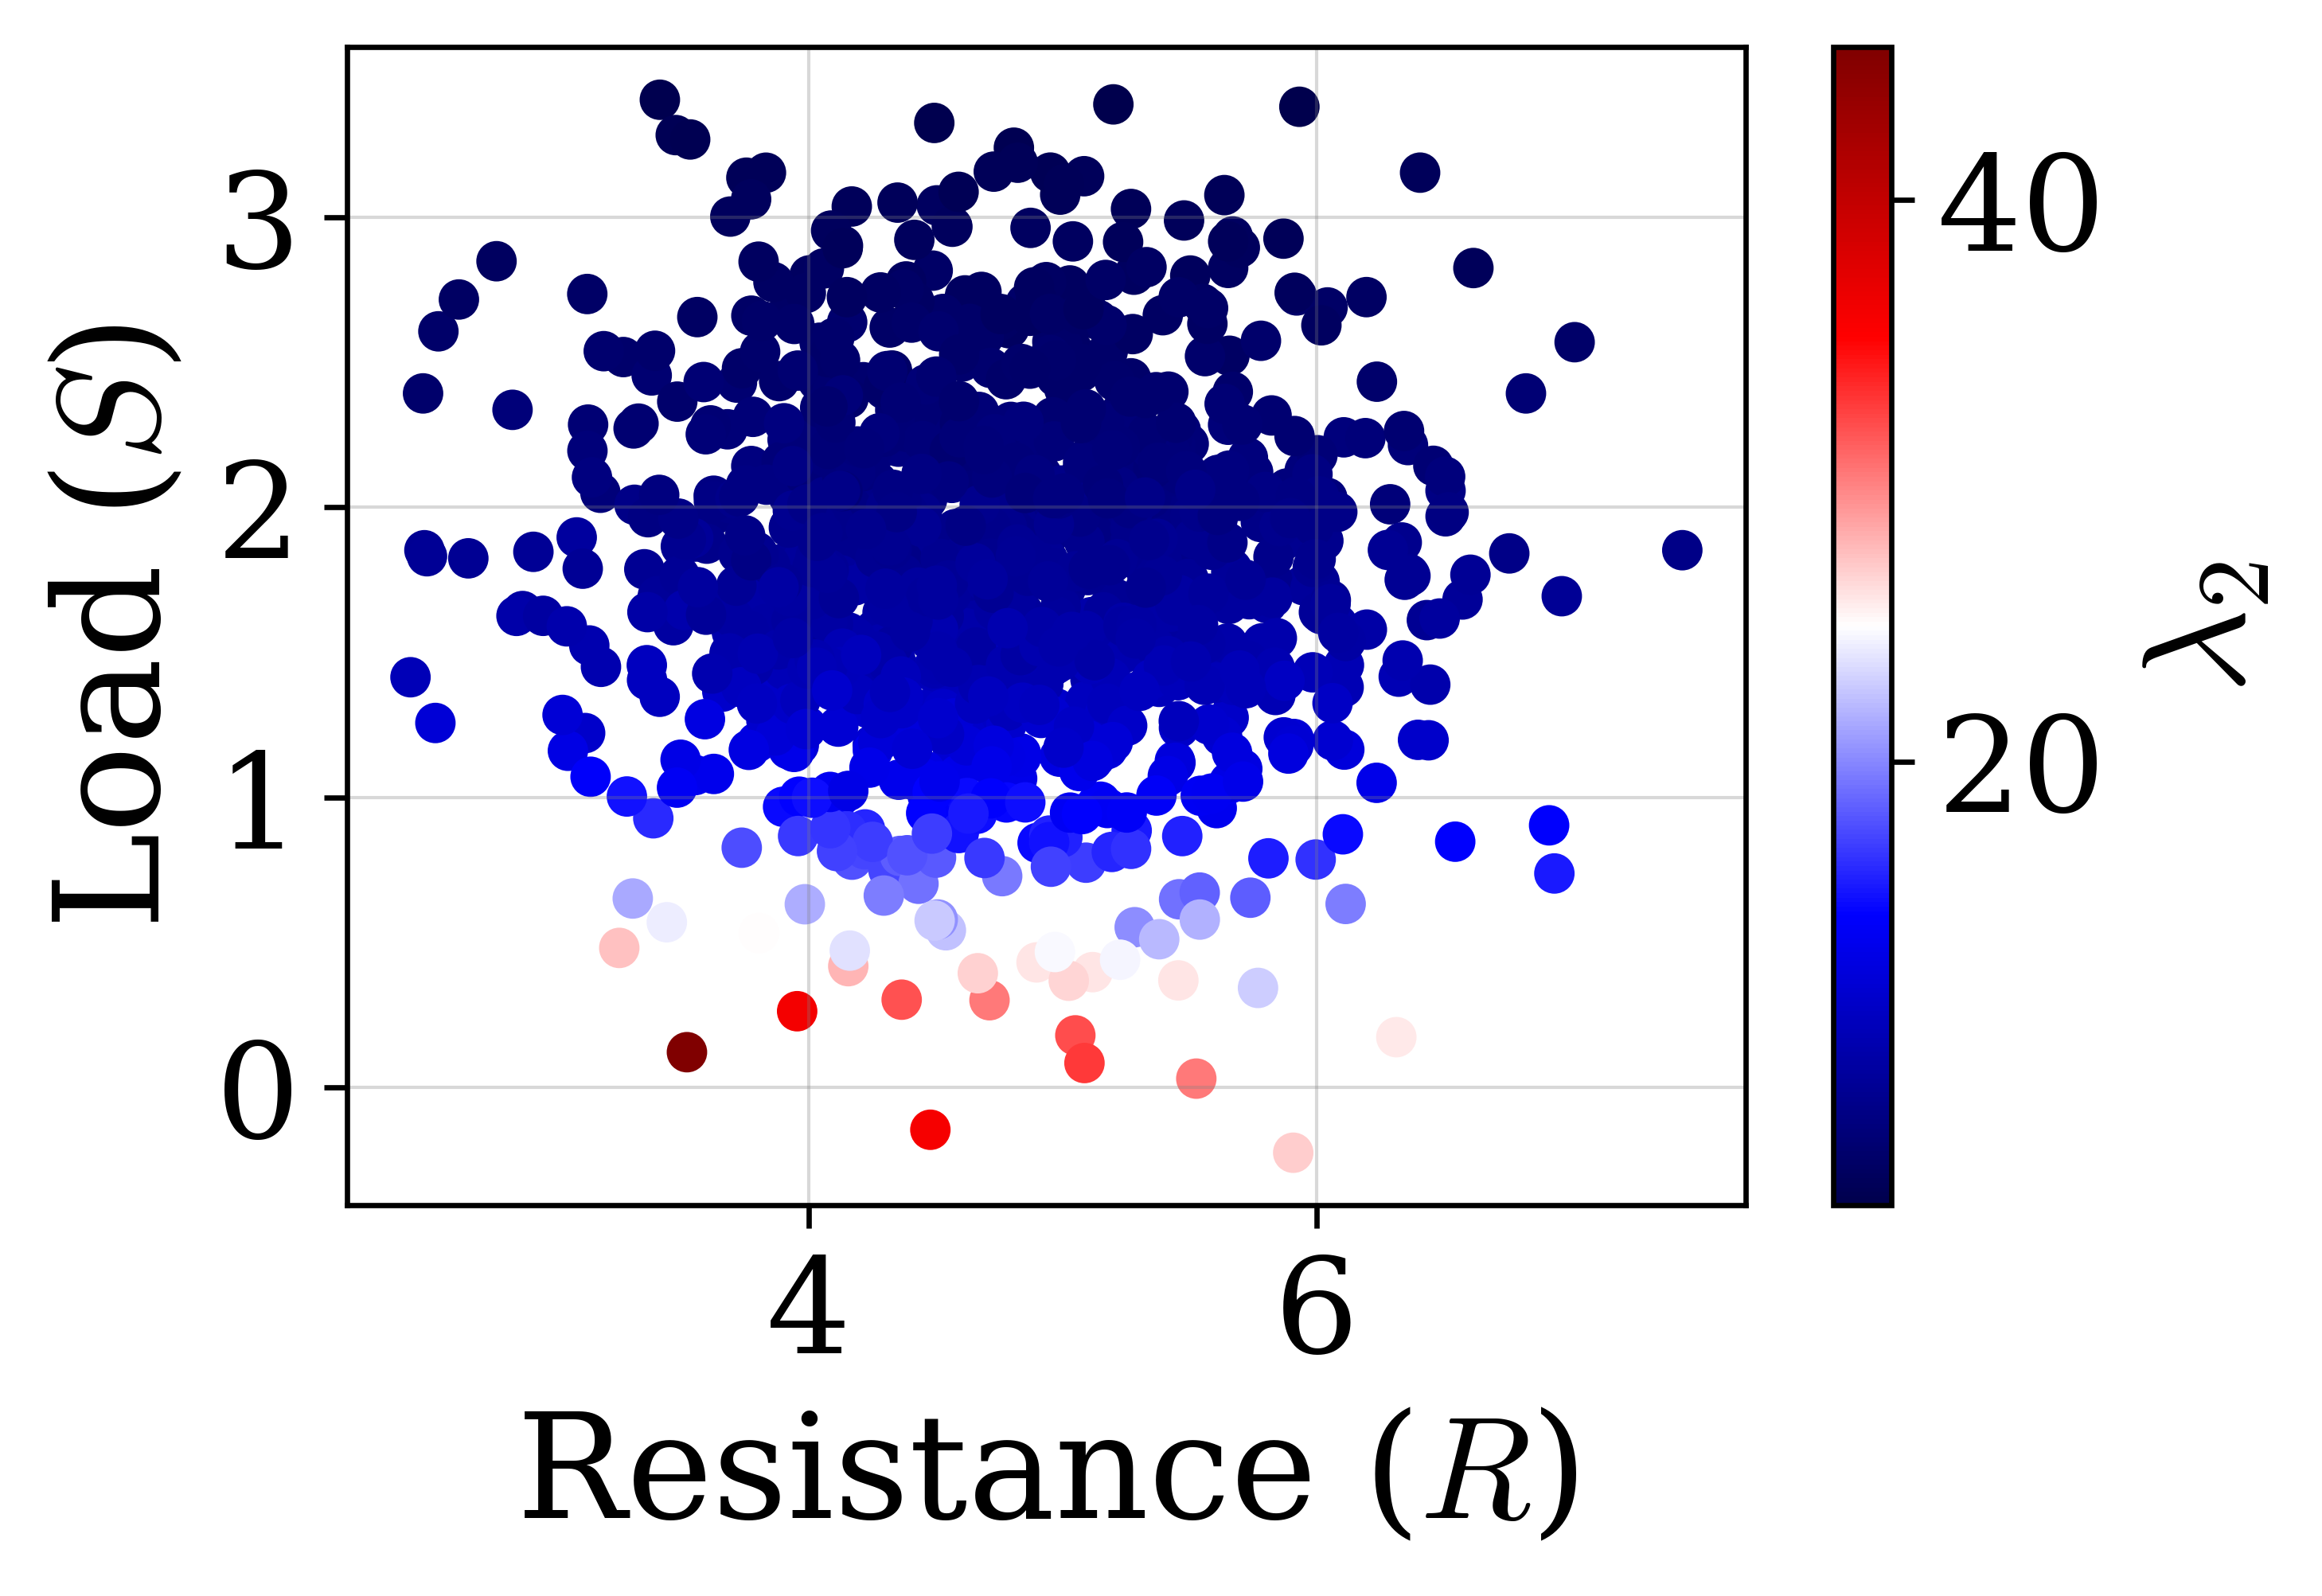
\includegraphics[
            width=\textwidth,
            height=0.667\textwidth,
            keepaspectratio
        ]{z_lambda_2_t-50.png}
        \caption{$\lambda_2$ ($t=50$)}
    \end{subfigure}
    \hfill
    \begin{subfigure}[b]{0.24\textwidth}
        \centering
        
\includegraphics[
            width=\textwidth,
            height=0.667\textwidth,
            keepaspectratio
        ]{z_lambda_3_t-50.png}
        \caption{$\lambda_3$ ($t=50$)}
    \end{subfigure}
    \hfill
    \begin{subfigure}[b]{0.24\textwidth}
        \centering
        
\includegraphics[
            width=\textwidth,
            height=0.667\textwidth,
            keepaspectratio
        ]{z_lambda_4_t-50.png}
        \caption{$\lambda_4$ ($t=50$)}
    \end{subfigure}

    \caption{Scatter plots of \textbf{R} and \textbf{S} realizations for GLAM parameters $\lambda_1$--$\lambda_4$ at $t=0$ and $t=50$.}
    \label{fig:toy_lambda_scatter_grid}
\end{figure}

%Assim ,é possível perceber que os valore de lamda 1 e 2 são sensíveis, enquanto 3 e 4 não alteram significativamente escala de alteração baixa. Isso corrobora a hiptese de não treinar 3 e 4. assim foi feito o treinamento com o seguinte resultado:

Based on this evidence, only $\lambda_1$ and $\lambda_2$ are selected as target variables for the surrogate model training. The performance of the resulting PCE metamodel is evaluated through the coefficient of determination, $R^2$, and the validation results are reported in Table~\ref{tab:validation_results}. The high $R^2$ values obtained for $\lambda_1$ and $\lambda_2$ across all time steps indicate excellent predictive accuracy, while the consistently low $R^2$ values for $\lambda_3$ and $\lambda_4$ further confirm their limited variability and support their exclusion from the training process.

\begin{table}[H]
\centering
\caption{Statistical validation results of the PCE metamodel at different time steps.}
\label{tab:validation_results}
\begin{tabular}{rrrrr}
\toprule
Time & $R^2$ ($\lambda_1$) & $R^2$ ($\lambda_2$) & $R^2$ ($\lambda_3$) & $R^2$ ($\lambda_4$) \\
\midrule
0 & 1.0000 & 0.9839 & 0.3858 & 0.3978 \\
10 & 1.0000 & 0.9887 & 0.4448 & 0.4226 \\
20 & 1.0000 & 0.9894 & 0.3713 & 0.3804 \\
30 & 1.0000 & 0.9833 & 0.3758 & 0.3624 \\
40 & 1.0000 & 0.9792 & 0.4081 & 0.3891 \\
50 & 1.0000 & 0.9908 & 0.3293 & 0.3757 \\
60 & 1.0000 & 0.9926 & 0.3102 & 0.3525 \\
70 & 1.0000 & 0.9853 & 0.2266 & 0.2852 \\
80 & 1.0000 & 0.9918 & 0.2277 & 0.2146 \\
90 & 1.0000 & 0.9820 & 0.1536 & 0.2200 \\
100 & 1.0000 & 0.9865 & 0.0638 & 0.1352 \\
\bottomrule
\end{tabular}
\end{table}

For the fixed realizations $r = 5.09$ and $s = 1.80$, four Polynomial Chaos Expansion (PCE) models were trained. Figure~\ref{fig:kde_comparison} presents the Kernel Density Estimation (KDE) comparison between the Ground Truth and the GLAM approximation obtained via PCE. For each realization, the GLAM–PCE response was evaluated and plotted at two distinct time periods, namely $t = 0$ and $t = 50$, allowing the assessment of the model’s ability to reproduce the probabilistic behavior of the reference solution over time.

\begin{figure}[H]
    \centering
    % --- Coluna 1: Tempo t=0 ---
    \begin{subfigure}[b]{0.38\textwidth}
        \centering
        % Substitua pelo nome do seu arquivo
        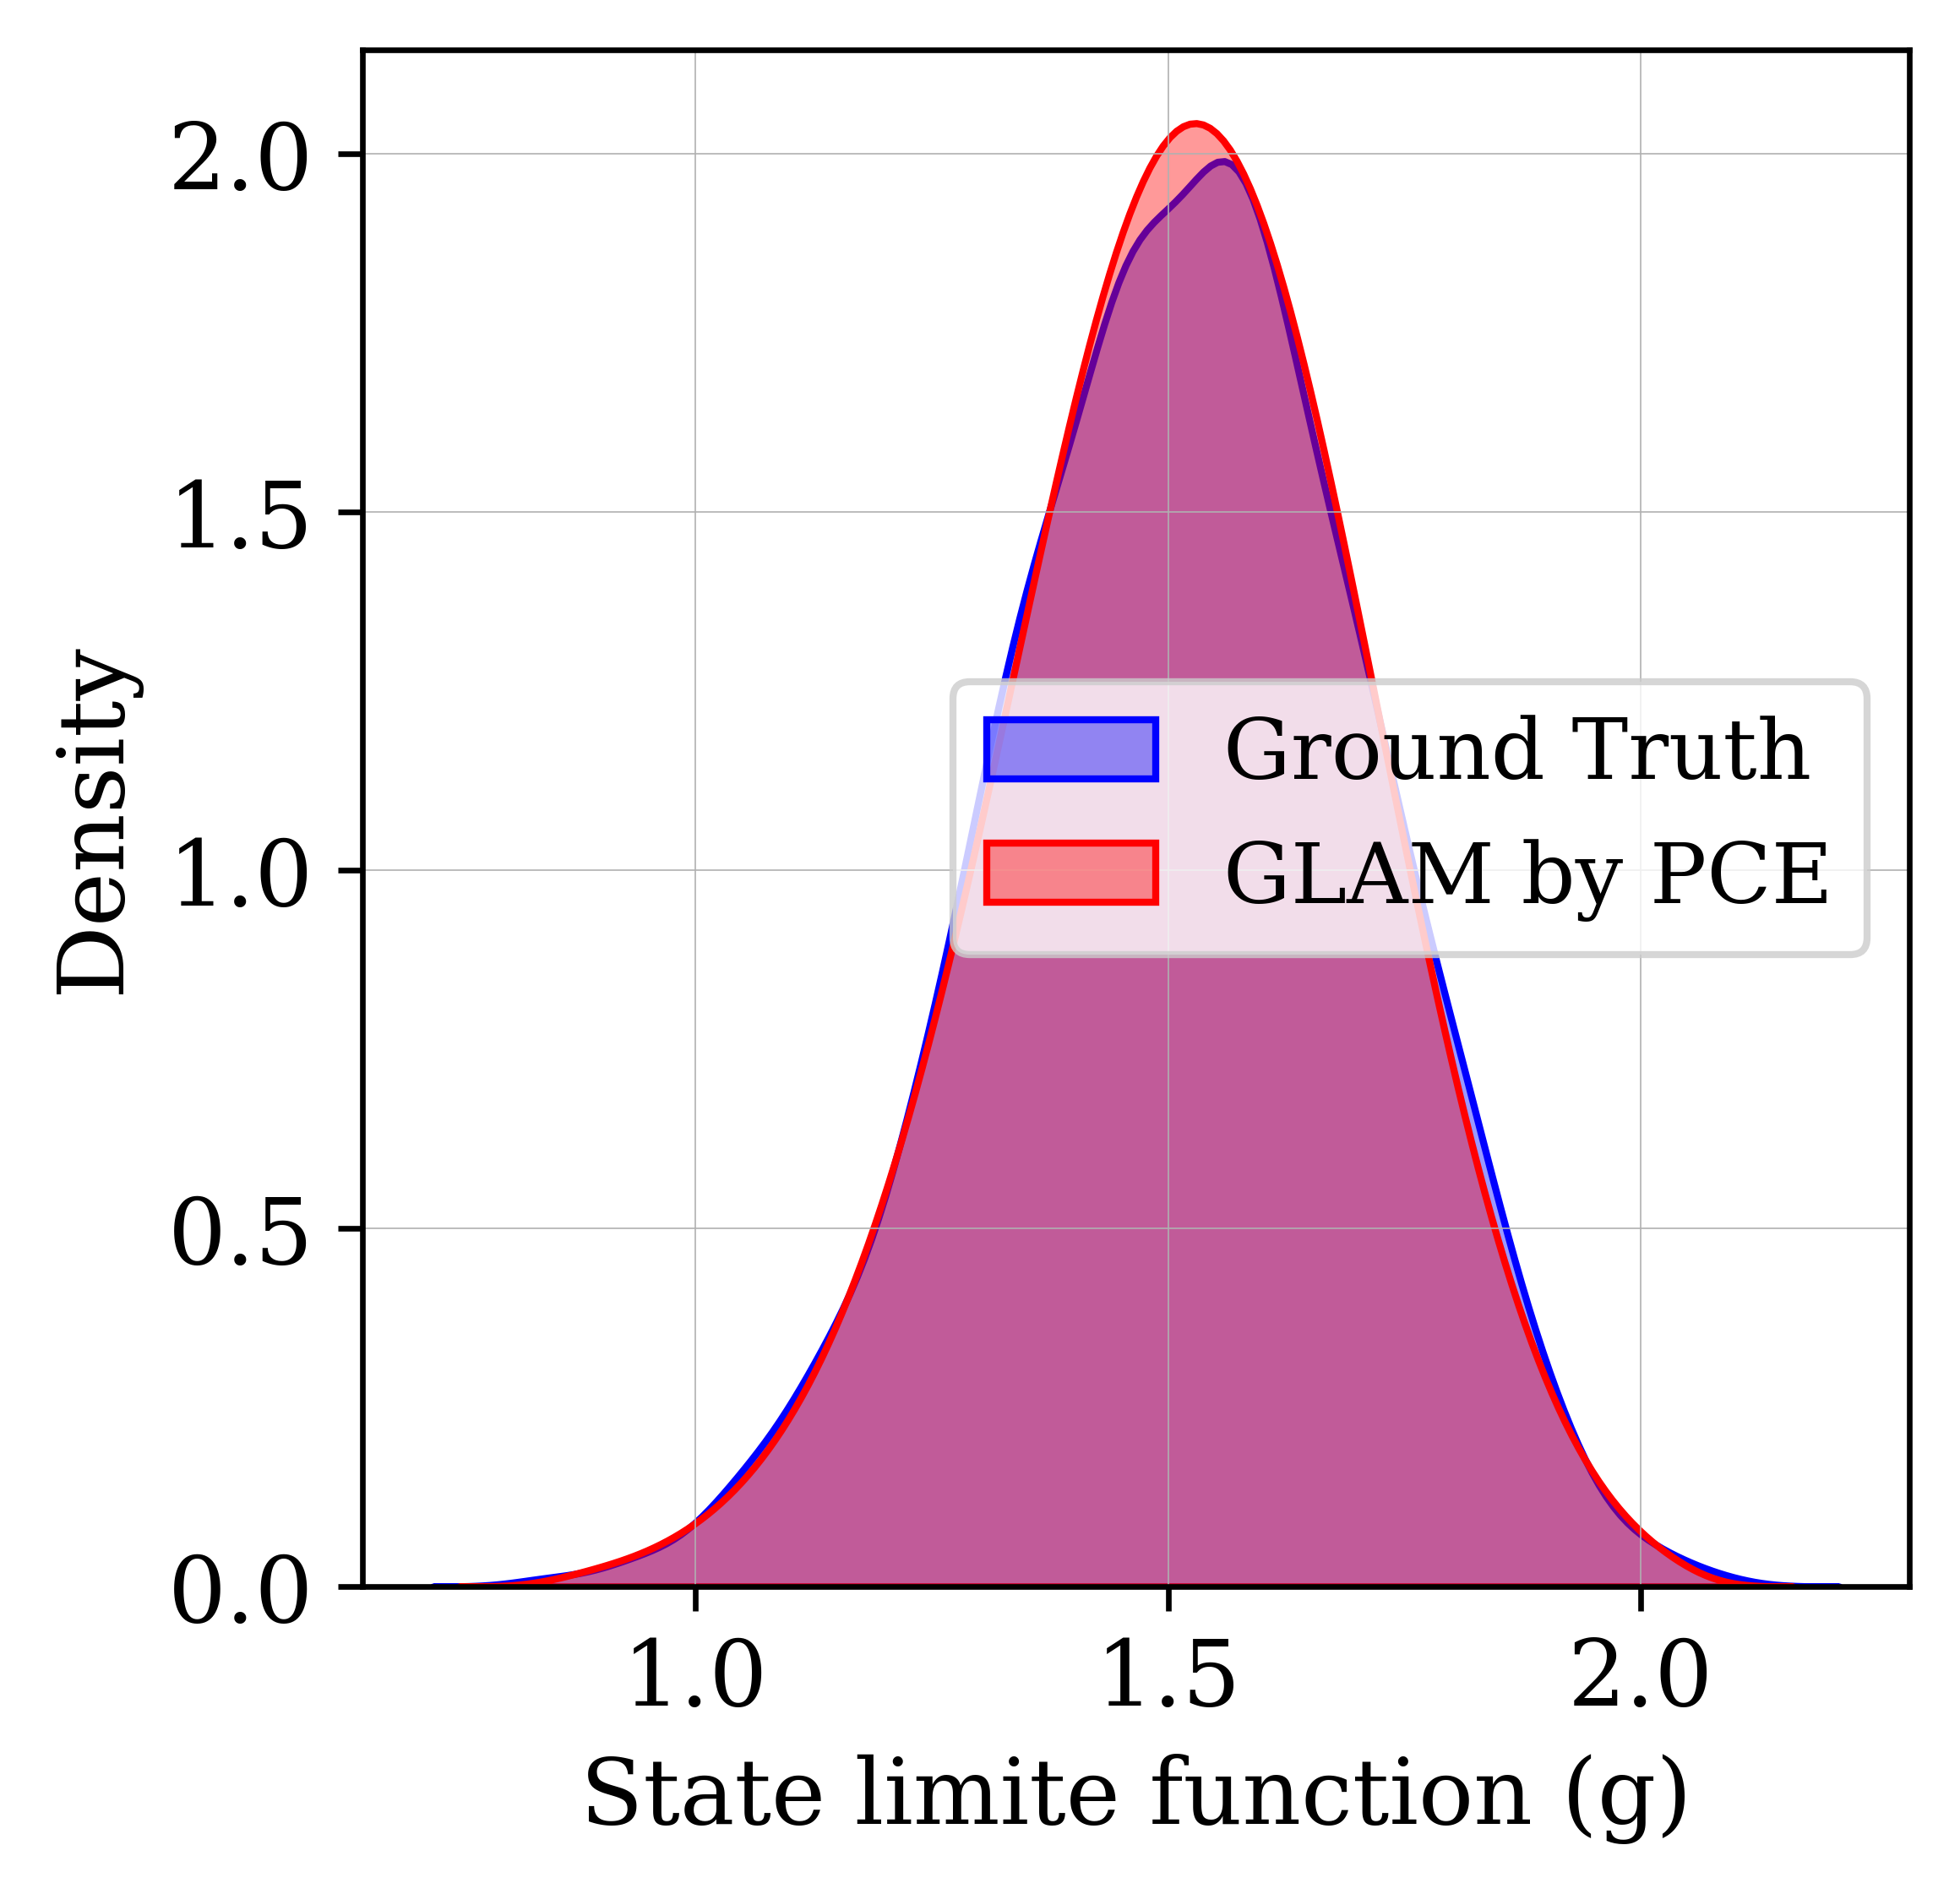
\includegraphics[width=\textwidth]{z_histogram_glam_versus_gt_t0_en.png}
        \caption{Time $t=0$}
        \label{fig:kde_t0}
    \end{subfigure}
    \hfill % O hfill empurra uma figura para a esquerda e outra para a direita
    % --- Coluna 2: Tempo t=50 ---
    \begin{subfigure}[b]{0.38\textwidth}
        \centering
        % Substitua pelo nome do seu arquivo
        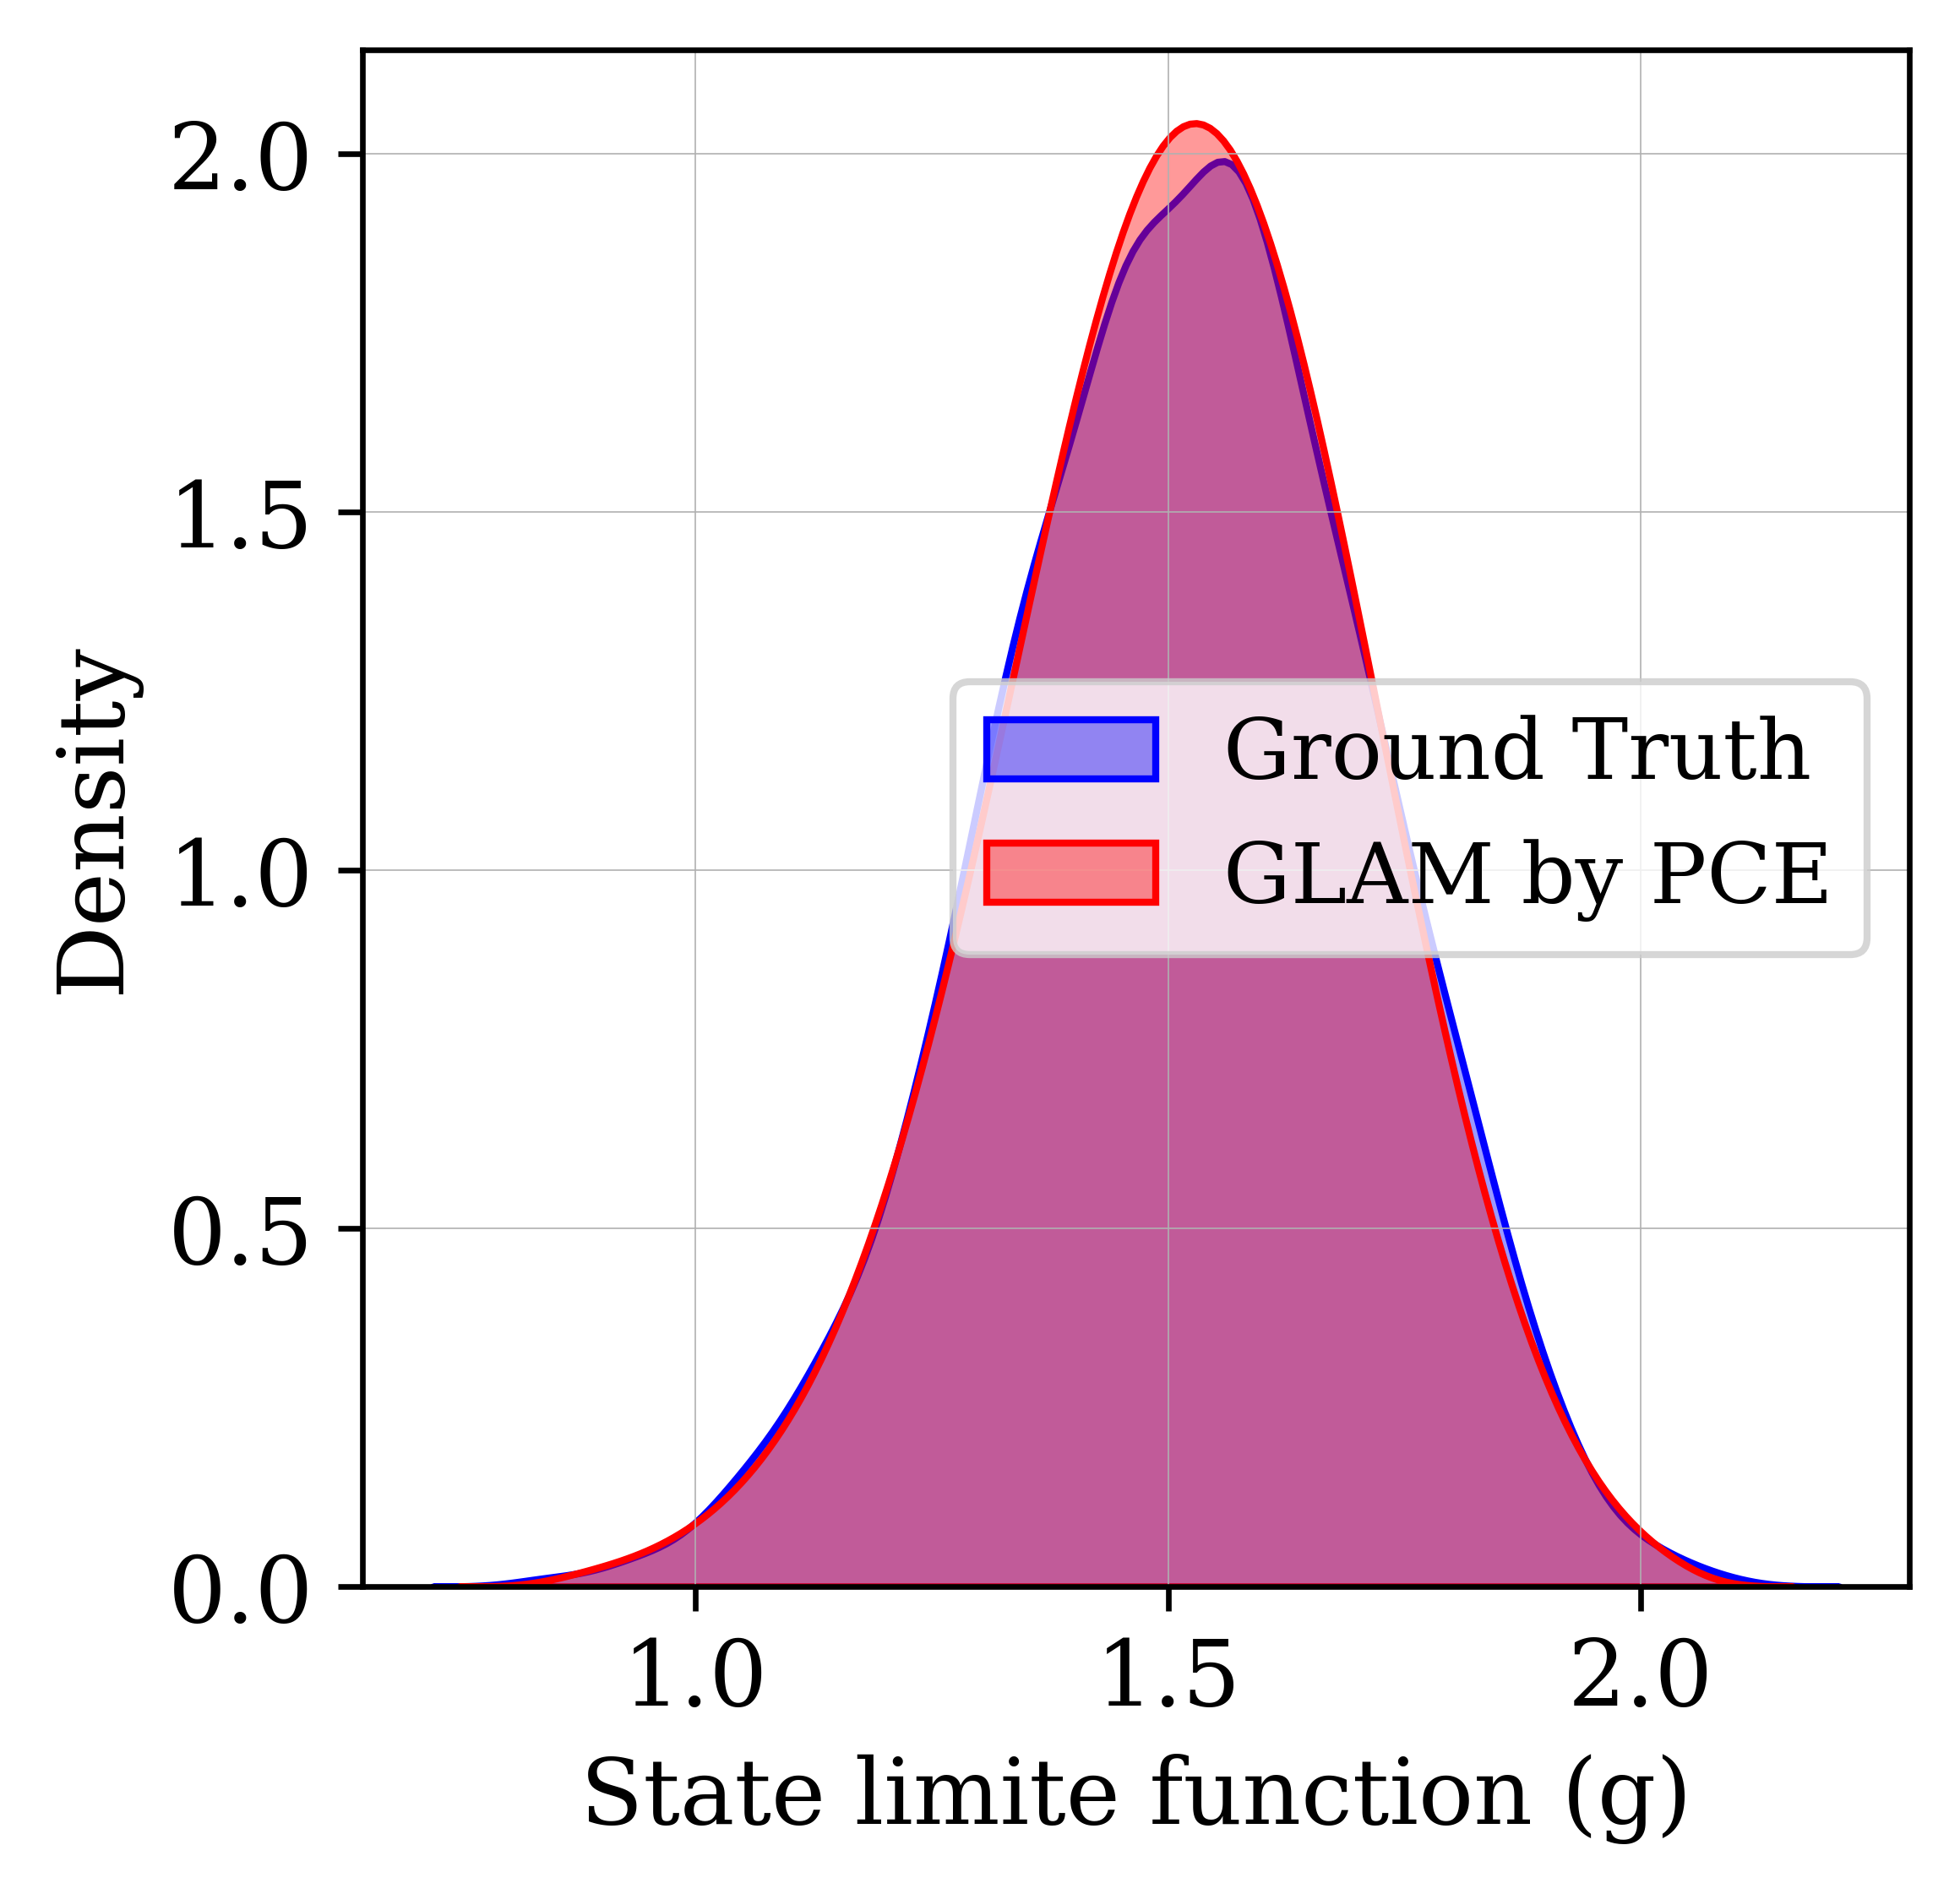
\includegraphics[width=\textwidth]{z_histogram_glam_versus_gt_t50_en.png}
        \caption{Time $t=50$}
        \label{fig:kde_t50}
    \end{subfigure}
    \caption{Comparison between Ground Truth and GLAM approximation using KDE. PCE models for the fixed realizations $r=5.09$ and $s=1.80$.}
    \label{fig:kde_comparison}
\end{figure}

The statistical similarity between the reference data (GT) and the values generated by the metamodel (GLAM) was assessed using non-parametric goodness-of-fit tests and quantile-based comparisons. Tables~\ref{tab:statistical_tests} and~\ref{tab:quantile_comparison} summarize the results of the hypothesis tests and the quantile comparison, respectively.

\begin{table}[H]
\centering
\caption{Results of the Kolmogorov--Smirnov and Anderson--Darling statistical tests for comparison between the reference data (GT) and the metamodel predictions (GLAM).}
\label{tab:statistical_tests}
\begin{tabular}{lcccc}
\hline
Test & Statistic & p-value & Significance level ($\alpha$) & Decision \\
\hline
Kolmogorov--Smirnov & 0.0108 & 0.9325 & 0.05 & Fail to reject $H_0$ \\
Anderson--Darling  & -0.6492 & 0.0025 & 0.05 & Reject $H_0$ \\
\hline
\end{tabular}
\end{table}

As shown in Table~\ref{tab:statistical_tests}, the Kolmogorov--Smirnov (KS) test does not reject the null hypothesis at the 5\% significance level, yielding a maximum distance of $D = 0.0108$. This result indicates an excellent global agreement between the empirical cumulative distribution functions of the reference data and the metamodel predictions. The KS test is primarily sensitive to the maximum discrepancy over the entire support of the distribution, making it well suited for assessing overall distributional similarity \cite{massey1951ks}.

In contrast, the Anderson--Darling (AD) test rejects the null hypothesis, indicating statistically significant differences between the samples. This outcome is attributed to the higher sensitivity of the AD test to discrepancies in the tails of the distribution, particularly in the presence of large sample sizes \cite{anderson1952ad, scholz1987ad}. Such behavior is well documented in the literature and does not necessarily imply poor global agreement between distributions.

To further investigate the origin of the discrepancy identified by the Anderson--Darling test, a quantile-based comparison was performed. The results are presented in Table~\ref{tab:quantile_comparison}.

\begin{table}[H]
\centering
\caption{Quantile comparison between the reference data (GT) and the metamodel predictions (GLAM).}
\label{tab:quantile_comparison}
\begin{tabular}{ccccc}
\hline
Quantile & GT & GLAM & Absolute difference & Relative difference (\%) \\
\hline
0.001 & 0.8995 & 0.9037 & 0.0042 & 0.47 \\
0.010 & 1.0387 & 1.0393 & 0.0006 & 0.06 \\
0.500 & 1.5222 & 1.5198 & 0.0024 & 0.16 \\
0.990 & 1.9374 & 1.9356 & 0.0018 & 0.09 \\
0.999 & 2.0529 & 2.0263 & 0.0266 & 1.30 \\
\hline
\end{tabular}
\end{table}

The quantile analysis reported in Table~\ref{tab:quantile_comparison} confirms the excellent agreement between the two datasets across nearly the entire distribution. Relative differences remain below 0.1\% up to the 99th percentile, indicating that the metamodel accurately reproduces the central and moderately extreme regions of the distribution. At the extreme quantile of 99.9\%, the relative discrepancy increases to approximately 1.3\%, which explains the rejection observed in the Anderson--Darling test due to its strong emphasis on tail behavior.

Overall, the combined evidence from the KS test, the AD test, and the quantile-based comparison demonstrates that the metamodel provides an accurate representation of the global distribution of the limit-state function, with only minor discrepancies confined to the extreme tails. Such discrepancies are commonly observed in surrogate-based modeling approaches and are generally considered acceptable in reliability and uncertainty quantification analyses, particularly when the primary interest lies in the global probabilistic response \cite{derkiureghian2009uq, sudret2008pce}.

In addition to the accuracy of the probabilistic predictions, the proposed emulator-based framework offers a substantial gain in computational efficiency. Table~\ref{tab:computational_time} compares the computational time required by the conventional approach and the surrogate-based emulator for the considered example. While the conventional procedure required approximately $48.75$ seconds, the emulator reduced the computational cost to only $0.66$ seconds, corresponding to a speed-up of more than two orders of magnitude. This result highlights the suitability of the proposed approach for real-time or large-scale reliability and RUL analyses.

\begin{table}[H]
\centering
\caption{Comparison of computational time between the conventional approach and the emulator-based approach.}
\label{tab:computational_time}
\begin{tabular}{l c}
\hline
\textbf{Method} & \textbf{Computational Time (s)} \\
\hline
Conventional approach & 48.75 \\
Emulator-based approach & 0.66 \\
\hline
\end{tabular}
\end{table}

Figure~\ref{fig:rul_results} presents the probabilistic outputs of the surrogate-based framework employed for Remaining Useful Life (RUL) assessment within a structural health monitoring context. The results illustrate the propagation of uncertainty from the limit state response to the final RUL estimation.

Figure~\ref{fig:kde_inspection_time} shows the Kernel Density Estimation (KDE) of the limit state function evaluated at the inspection time of 35 years, adopted here as a representative example. This distribution characterizes the uncertainty associated with the system condition at the inspection instant, capturing both the inherent variability of the stochastic inputs and the approximation effects introduced by the surrogate model.

The probability density function of the time to failure is presented in Figure~\ref{fig:kde_time_to_failure}. This distribution is obtained by identifying the time instant at which the limit state function approaches zero, providing a probabilistic description of the system lifetime and enabling a reliability-based interpretation of failure occurrence.

Finally, Figure~\ref{fig:kde_rul} presents the resulting RUL distribution, computed as the difference between the estimated time to failure and the inspection time. This distribution consolidates the propagated uncertainties and represents the key outcome for predictive maintenance and risk-informed decision-making.

\begin{figure}[H]
    \centering

    \begin{subfigure}[b]{0.32\textwidth}
        \centering
        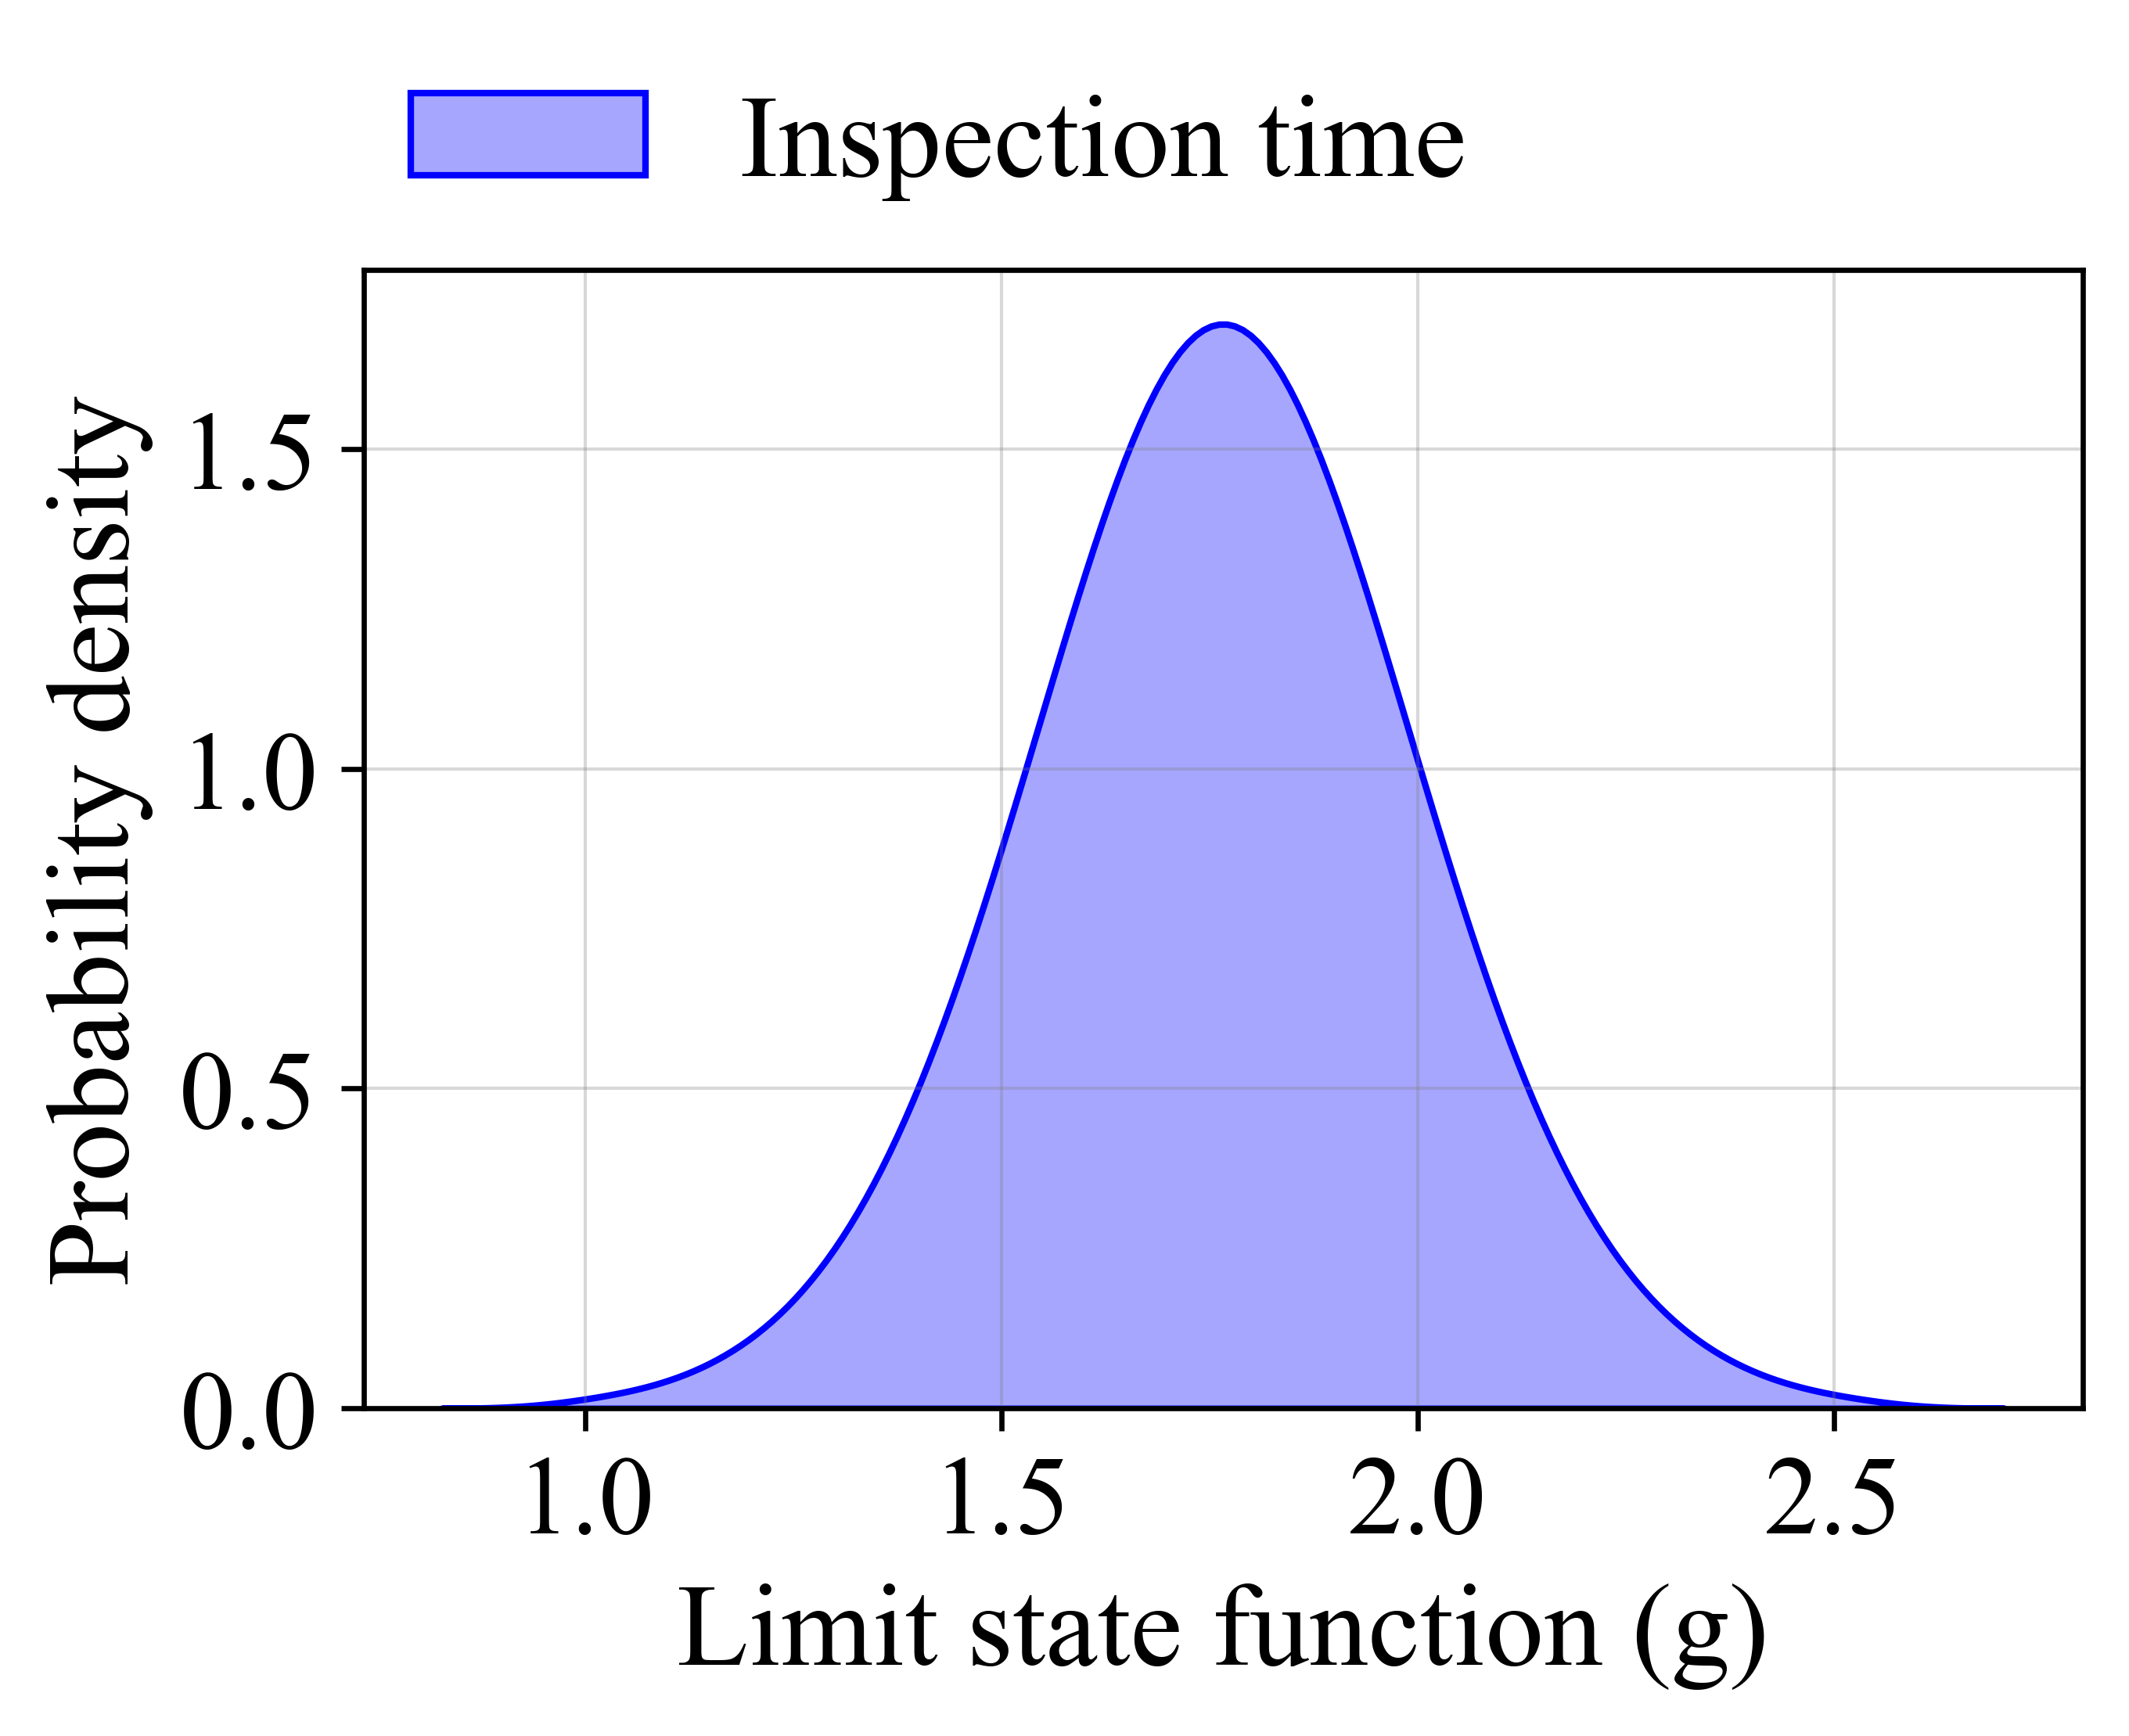
\includegraphics[
            height=4.0cm,
            keepaspectratio
        ]{z_kde_inspection_time.png}
        \caption{KDE of the limit state function at the inspection time.}
        \label{fig:kde_inspection_time}
    \end{subfigure}
    \hfill
    \begin{subfigure}[b]{0.32\textwidth}
        \centering
        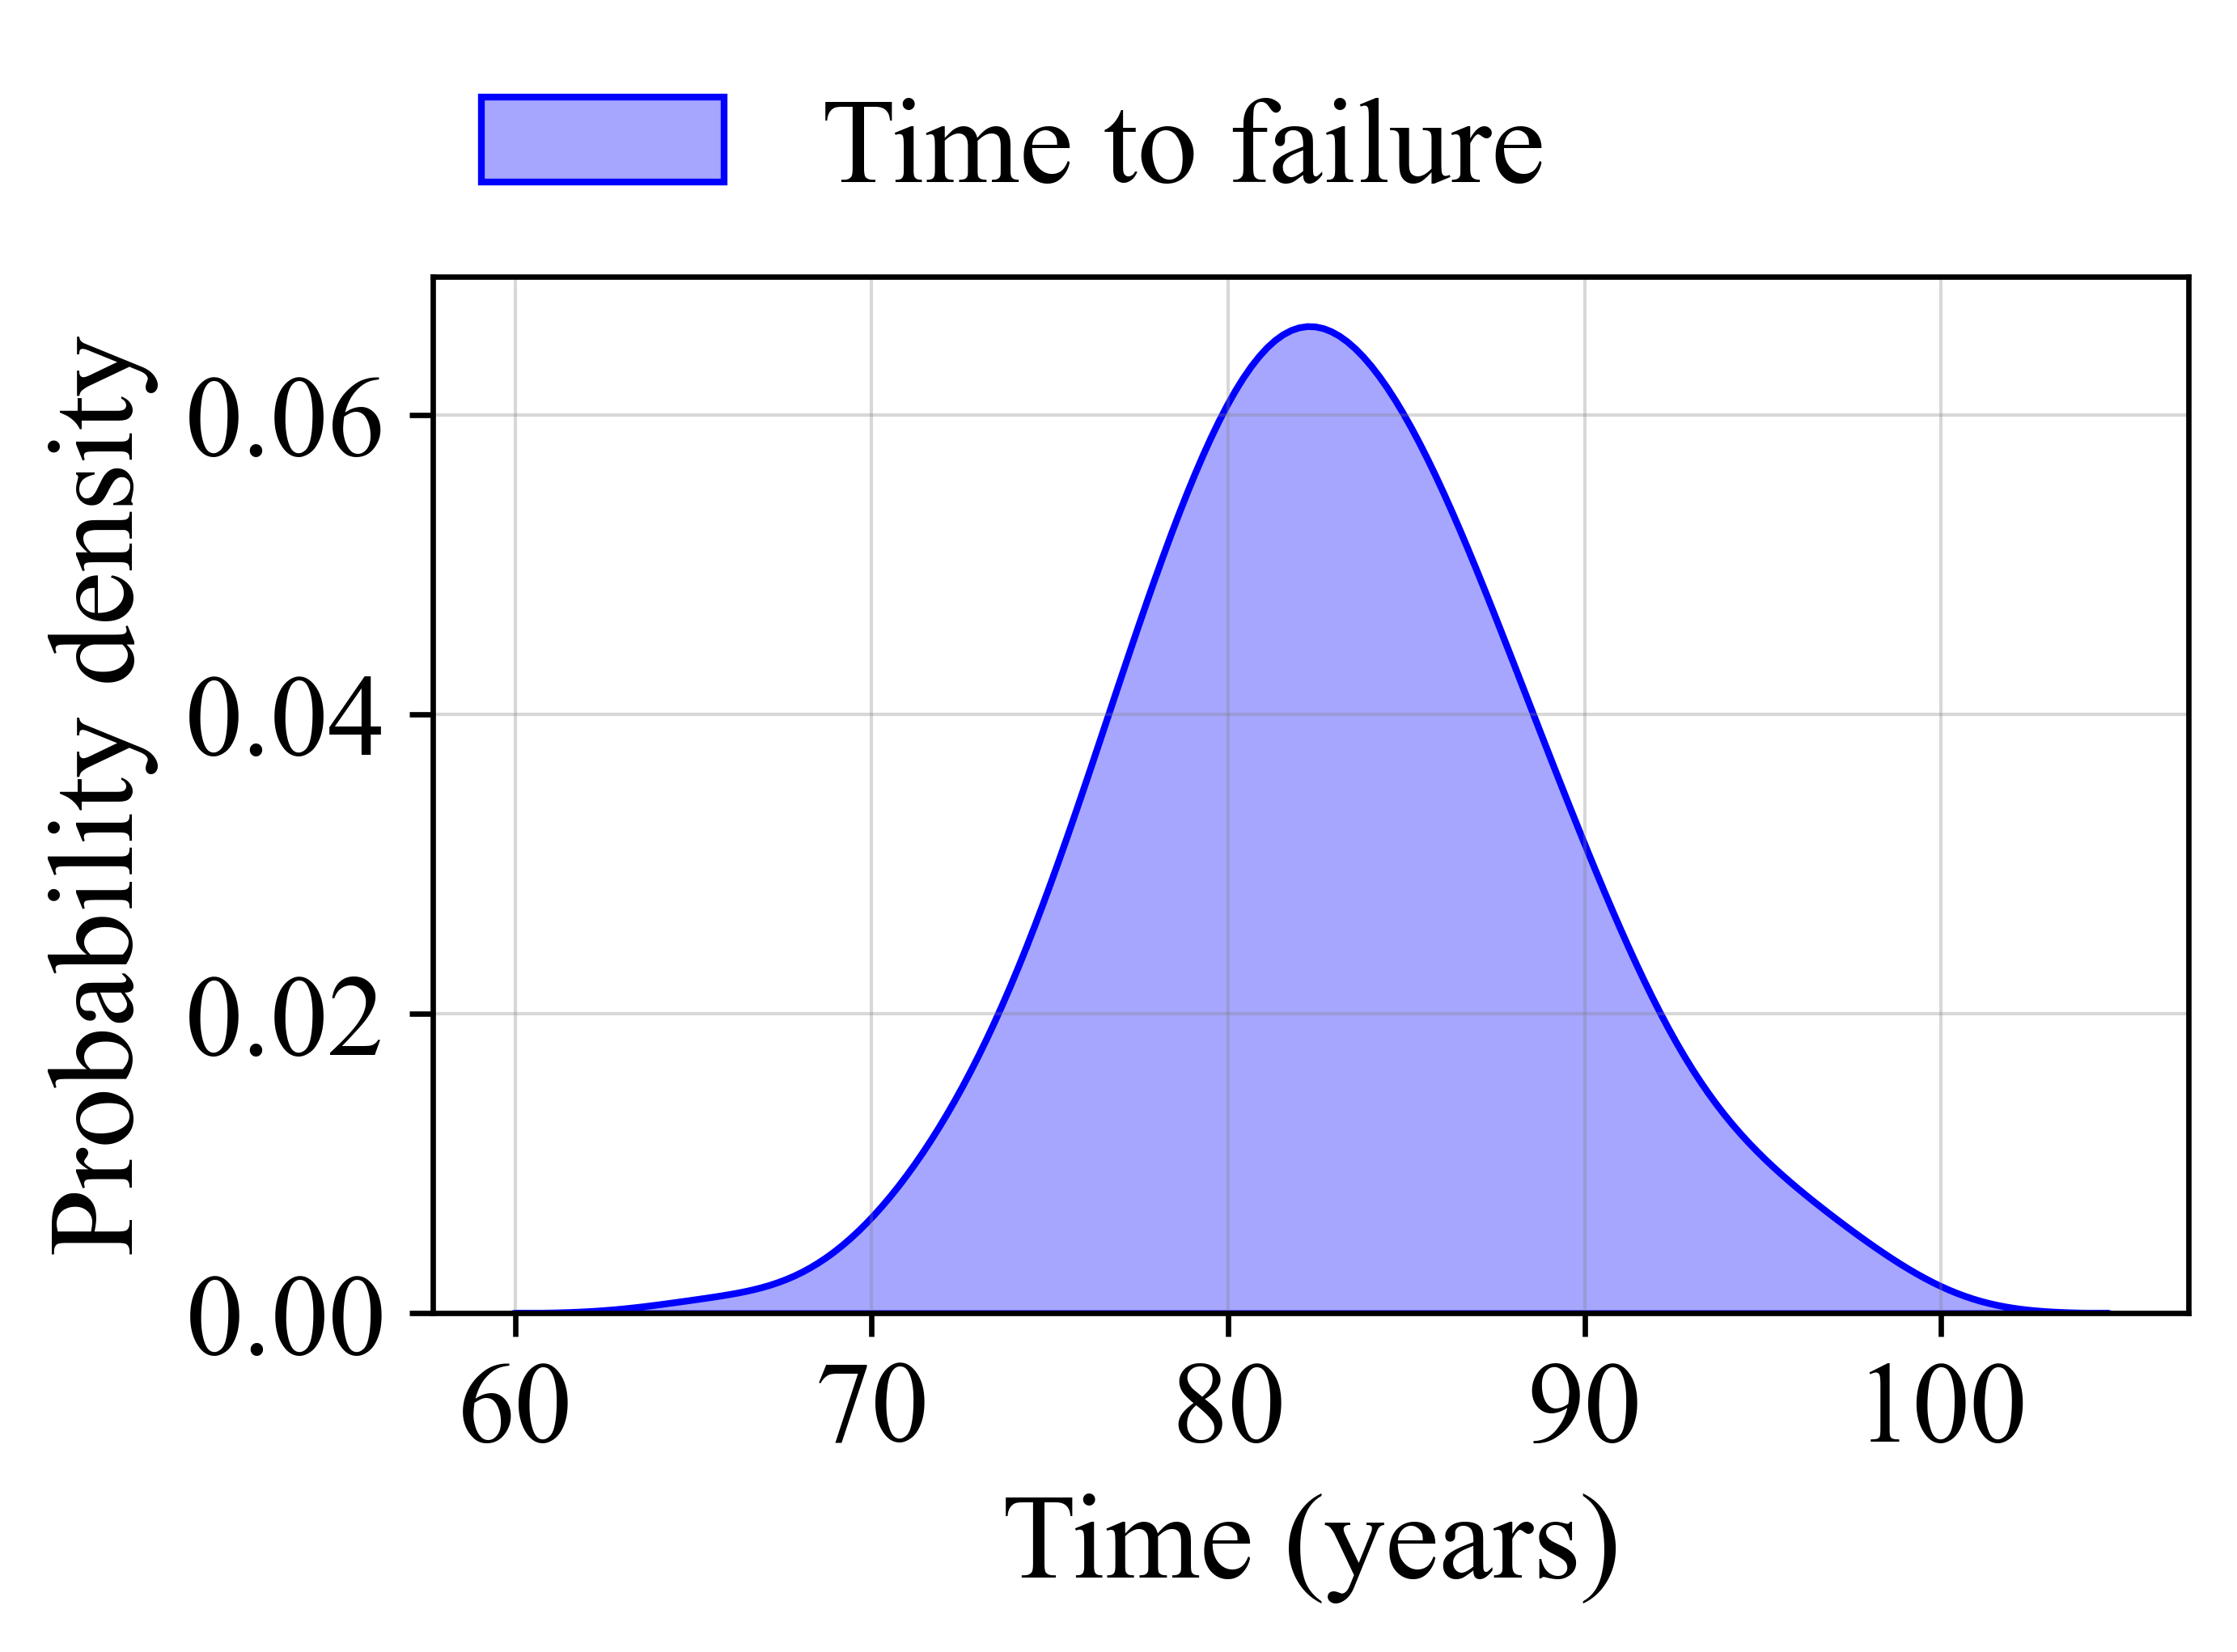
\includegraphics[
            height=4.0cm,
            keepaspectratio
        ]{z_kde_time_to_failure.png}
        \caption{Probability density of the time to failure.}
        \label{fig:kde_time_to_failure}
    \end{subfigure}
    \hfill
    \begin{subfigure}[b]{0.32\textwidth}
        \centering
        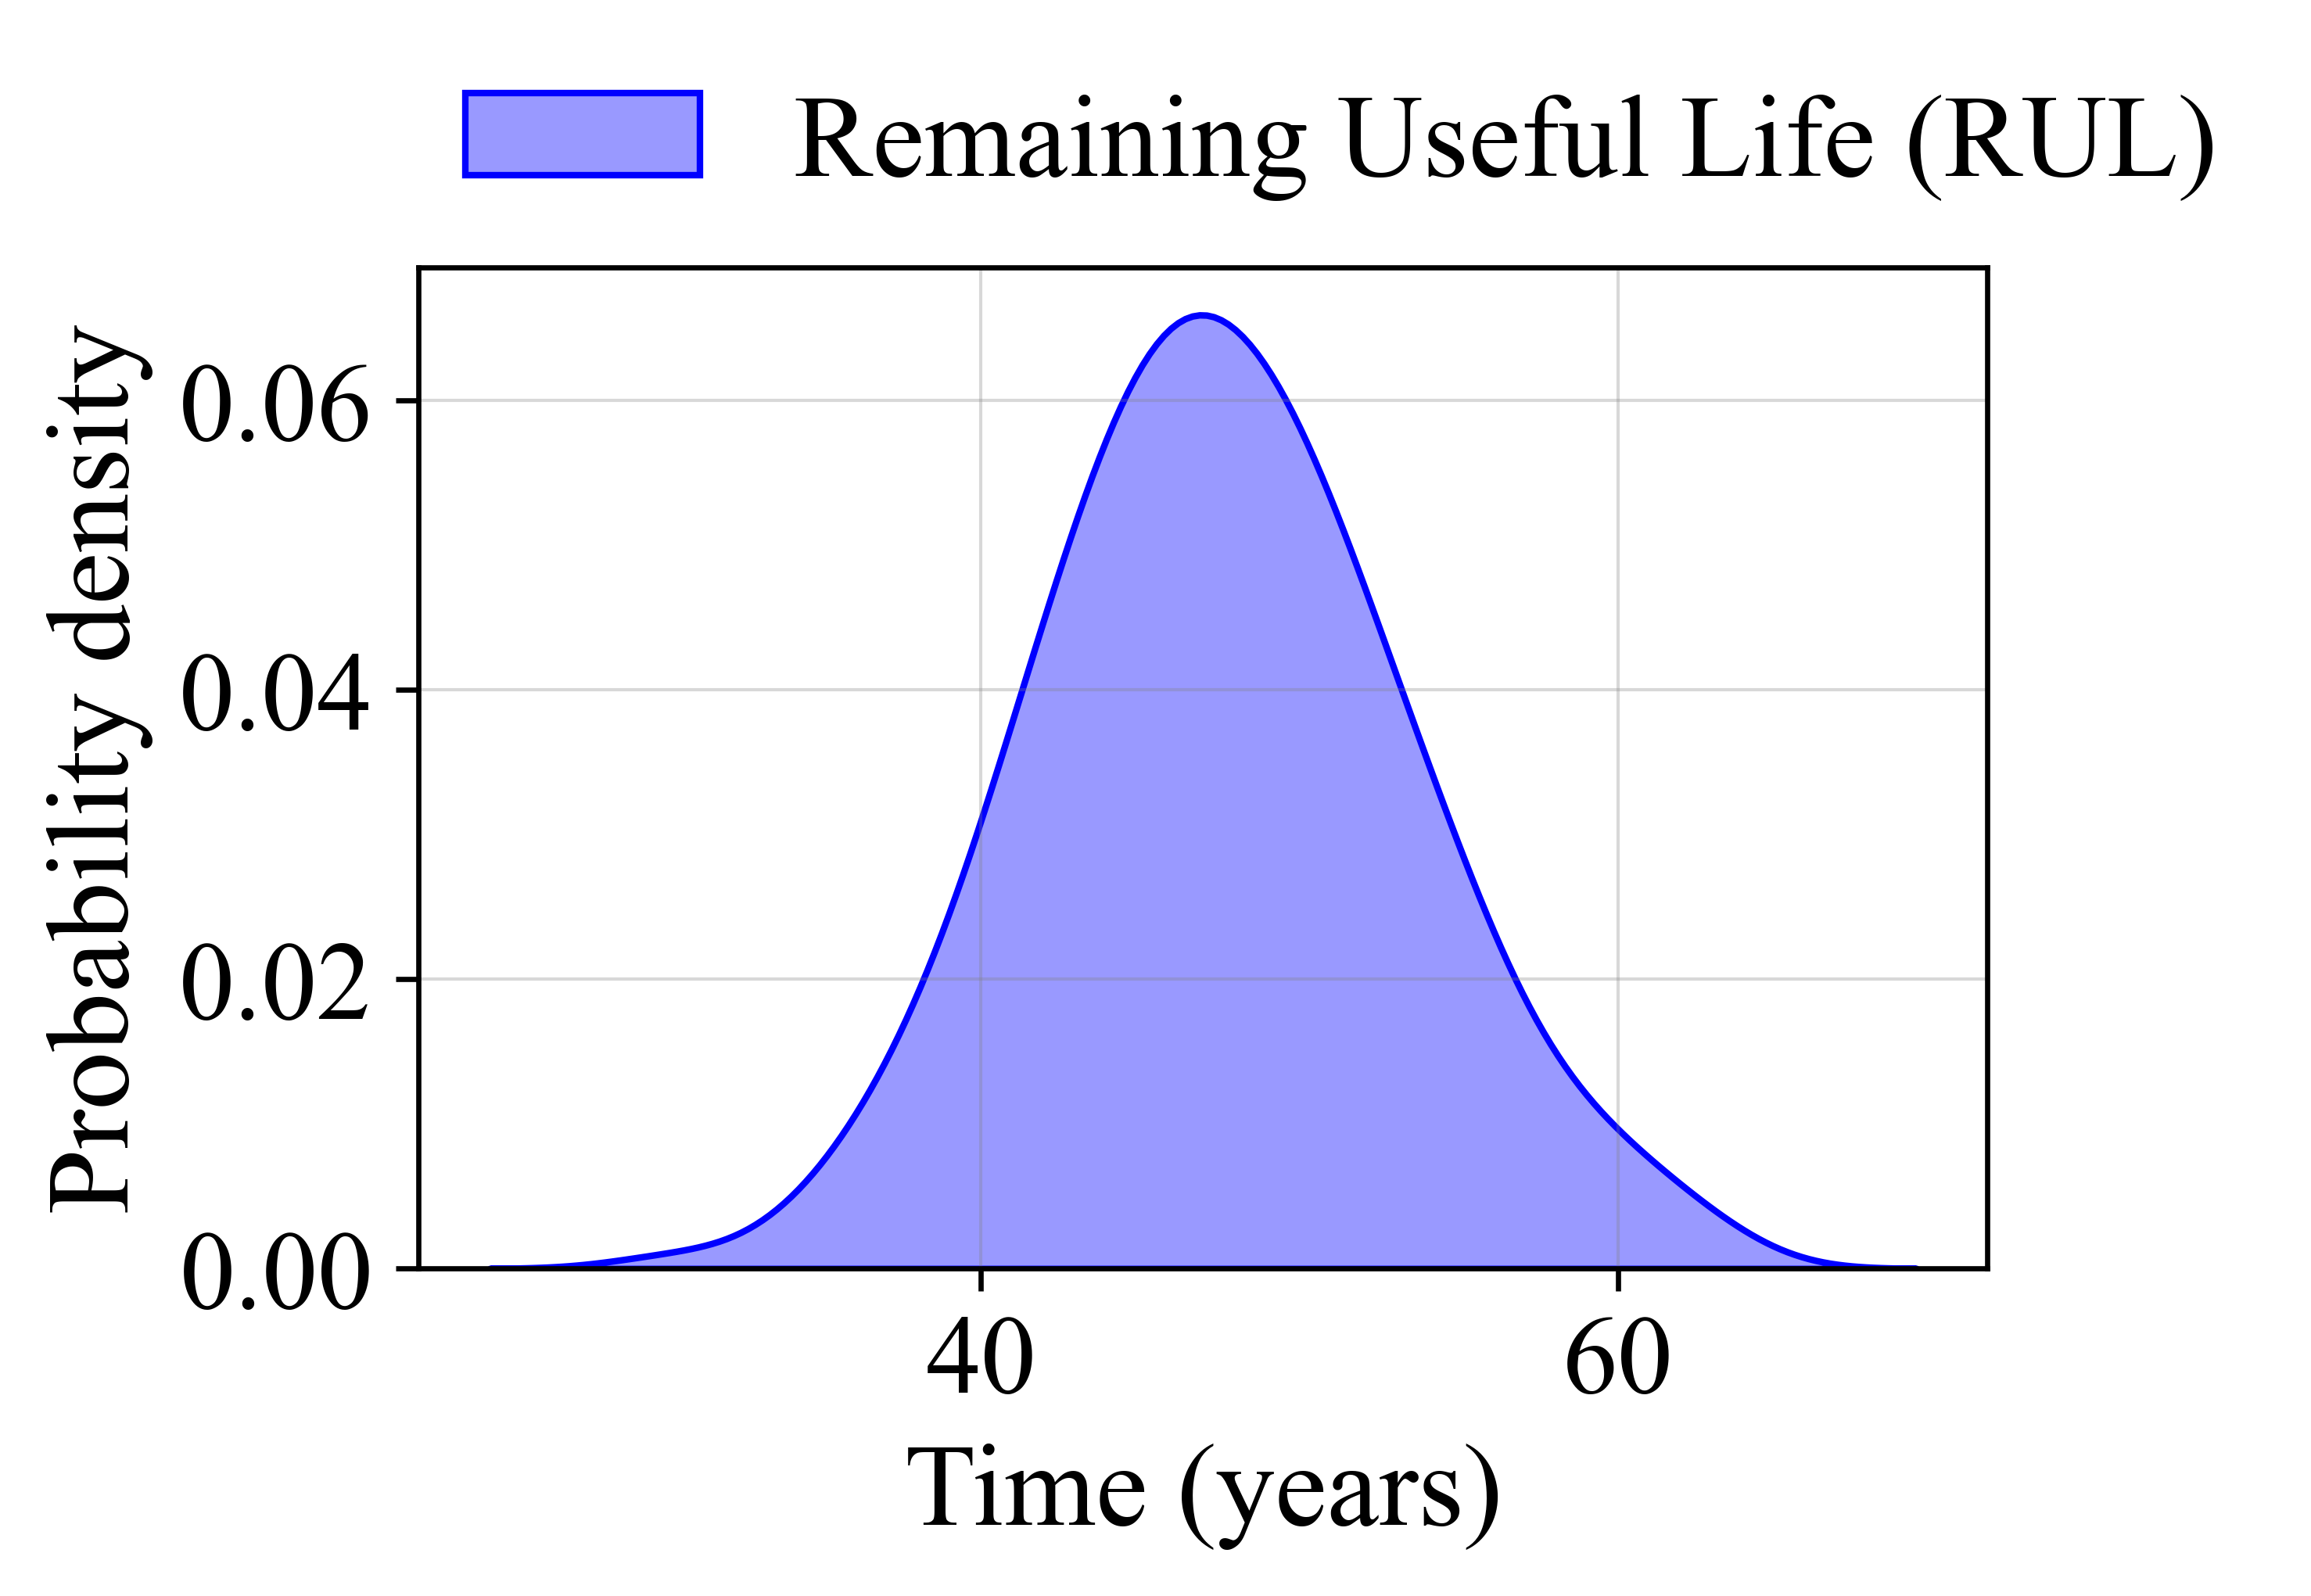
\includegraphics[
            height=4.0cm,
            keepaspectratio
        ]{z_kde_rul.png}
        \caption{KDE of the Remaining Useful Life (RUL).}
        \label{fig:kde_rul}
    \end{subfigure}

    \caption{Probabilistic results obtained from the surrogate-based framework for Remaining Useful Life (RUL) estimation: (a) distribution of the limit state function at the inspection time, (b) distribution of the time to failure, and (c) resulting RUL distribution.}
    \label{fig:rul_results}
\end{figure}

To further support decision-making under uncertainty, risk-based metrics were derived from the Remaining Useful Life (RUL) distribution, namely the Value-at-Risk (VaR) and the Conditional Value-at-Risk (CVaR). While the full probabilistic characterization of RUL provides comprehensive insight into the system behavior, these scalar metrics offer conservative indicators focused on adverse scenarios, which are particularly relevant for maintenance planning and reliability-based decision processes.

The VaR at confidence level $\alpha$ represents the lower quantile of the RUL distribution, indicating the minimum remaining life that can be expected with a confidence level of $(1-\alpha)$. In contrast, the CVaR corresponds to the expected RUL conditioned on values below the VaR threshold, explicitly accounting for tail behavior and providing a more conservative measure of risk.

In this study, both metrics were computed for $\alpha = 5\%$ using the surrogate-based RUL samples. The results are summarized in Table~\ref{tab:var_cvar_rul}. The relatively small difference between VaR and CVaR suggests limited tail severity, indicating that even under unfavorable conditions the predicted remaining life does not exhibit abrupt degradation. This behavior reinforces the robustness of the proposed surrogate framework for probabilistic RUL assessment and its suitability for reliability-informed maintenance decision-making.

\begin{table}[H]
\centering
\caption{Risk-based metrics derived from the RUL distribution for $\alpha = 5\%$.}
\label{tab:var_cvar_rul}
\begin{tabular}{lc}
\hline
\textbf{Metric} & \textbf{Value} \\
\hline
VaR$_{5\%}$ & 38.38 \\
CVaR$_{5\%}$ & 36.42 \\
\hline
\end{tabular}
\end{table}





\subsubsection{Machine Learning}

Building upon the discrete time-step analysis performed via PCE, a machine learning approach was adopted to enable the continuous prediction of the GLAM parameters $\lambda_1$ and $\lambda_2$ throughout the structural service life. While the PCE models provide accurate predictions at fixed time intervals, an Artificial Neural Network (ANN) was implemented to generalize this behavior, allowing for the estimation of the parameters at any arbitrary time $t \in [0, 100]$ years.

To train the ANN, a comprehensive synthetic dataset comprising 11,000 samples was generated using the previously validated PCE metamodels. The input space was sampled based on the probability distributions of the resistance $R$ and load $S$ defined in Table~\ref{tab:random_variables_parameters}, combined with time values uniformly distributed over the analysis horizon.

The network was trained to map the input vector $\mathbf{x} = \{R, S, t\}$ to the output vector $\mathbf{y} = \{\lambda_1, \lambda_2\}$. The dataset was randomly partitioned into training and testing subsets to evaluate the model's generalization capability and avoid overfitting.

Figure~\ref{fig:z_temporal_evolution_ann_with_points_en.pn} illustrates the temporal evolution of the GLAM parameters $\lambda_1$ and $\lambda_2$ over the 100-year service life, predicted by the trained ANN for a representative scenario ($r=5.09$, $s=1.80$). The plot demonstrates the network's ability to act as a continuous interpolator, smoothly reconstructing the degradation trajectory between the discrete time steps originally evaluated by the PCE model. The coherent behavior of the curves, free from numerical noise or discontinuities, confirms that the ANN effectively learned the underlying physics of the time-dependent degradation process.

Quantitatively, the model demonstrated excellent predictive accuracy, achieving coefficients of determination ($R^2$) of 0.9976 for $\lambda_1$ and 0.9844 for $\lambda_2$. These high correlation metrics, combined with the visual smoothness of the temporal predictions, validate the ANN as a robust and computationally efficient tool for continuous reliability assessment at any arbitrary time point within the analysis horizon.

\begin{figure}
    \centering
    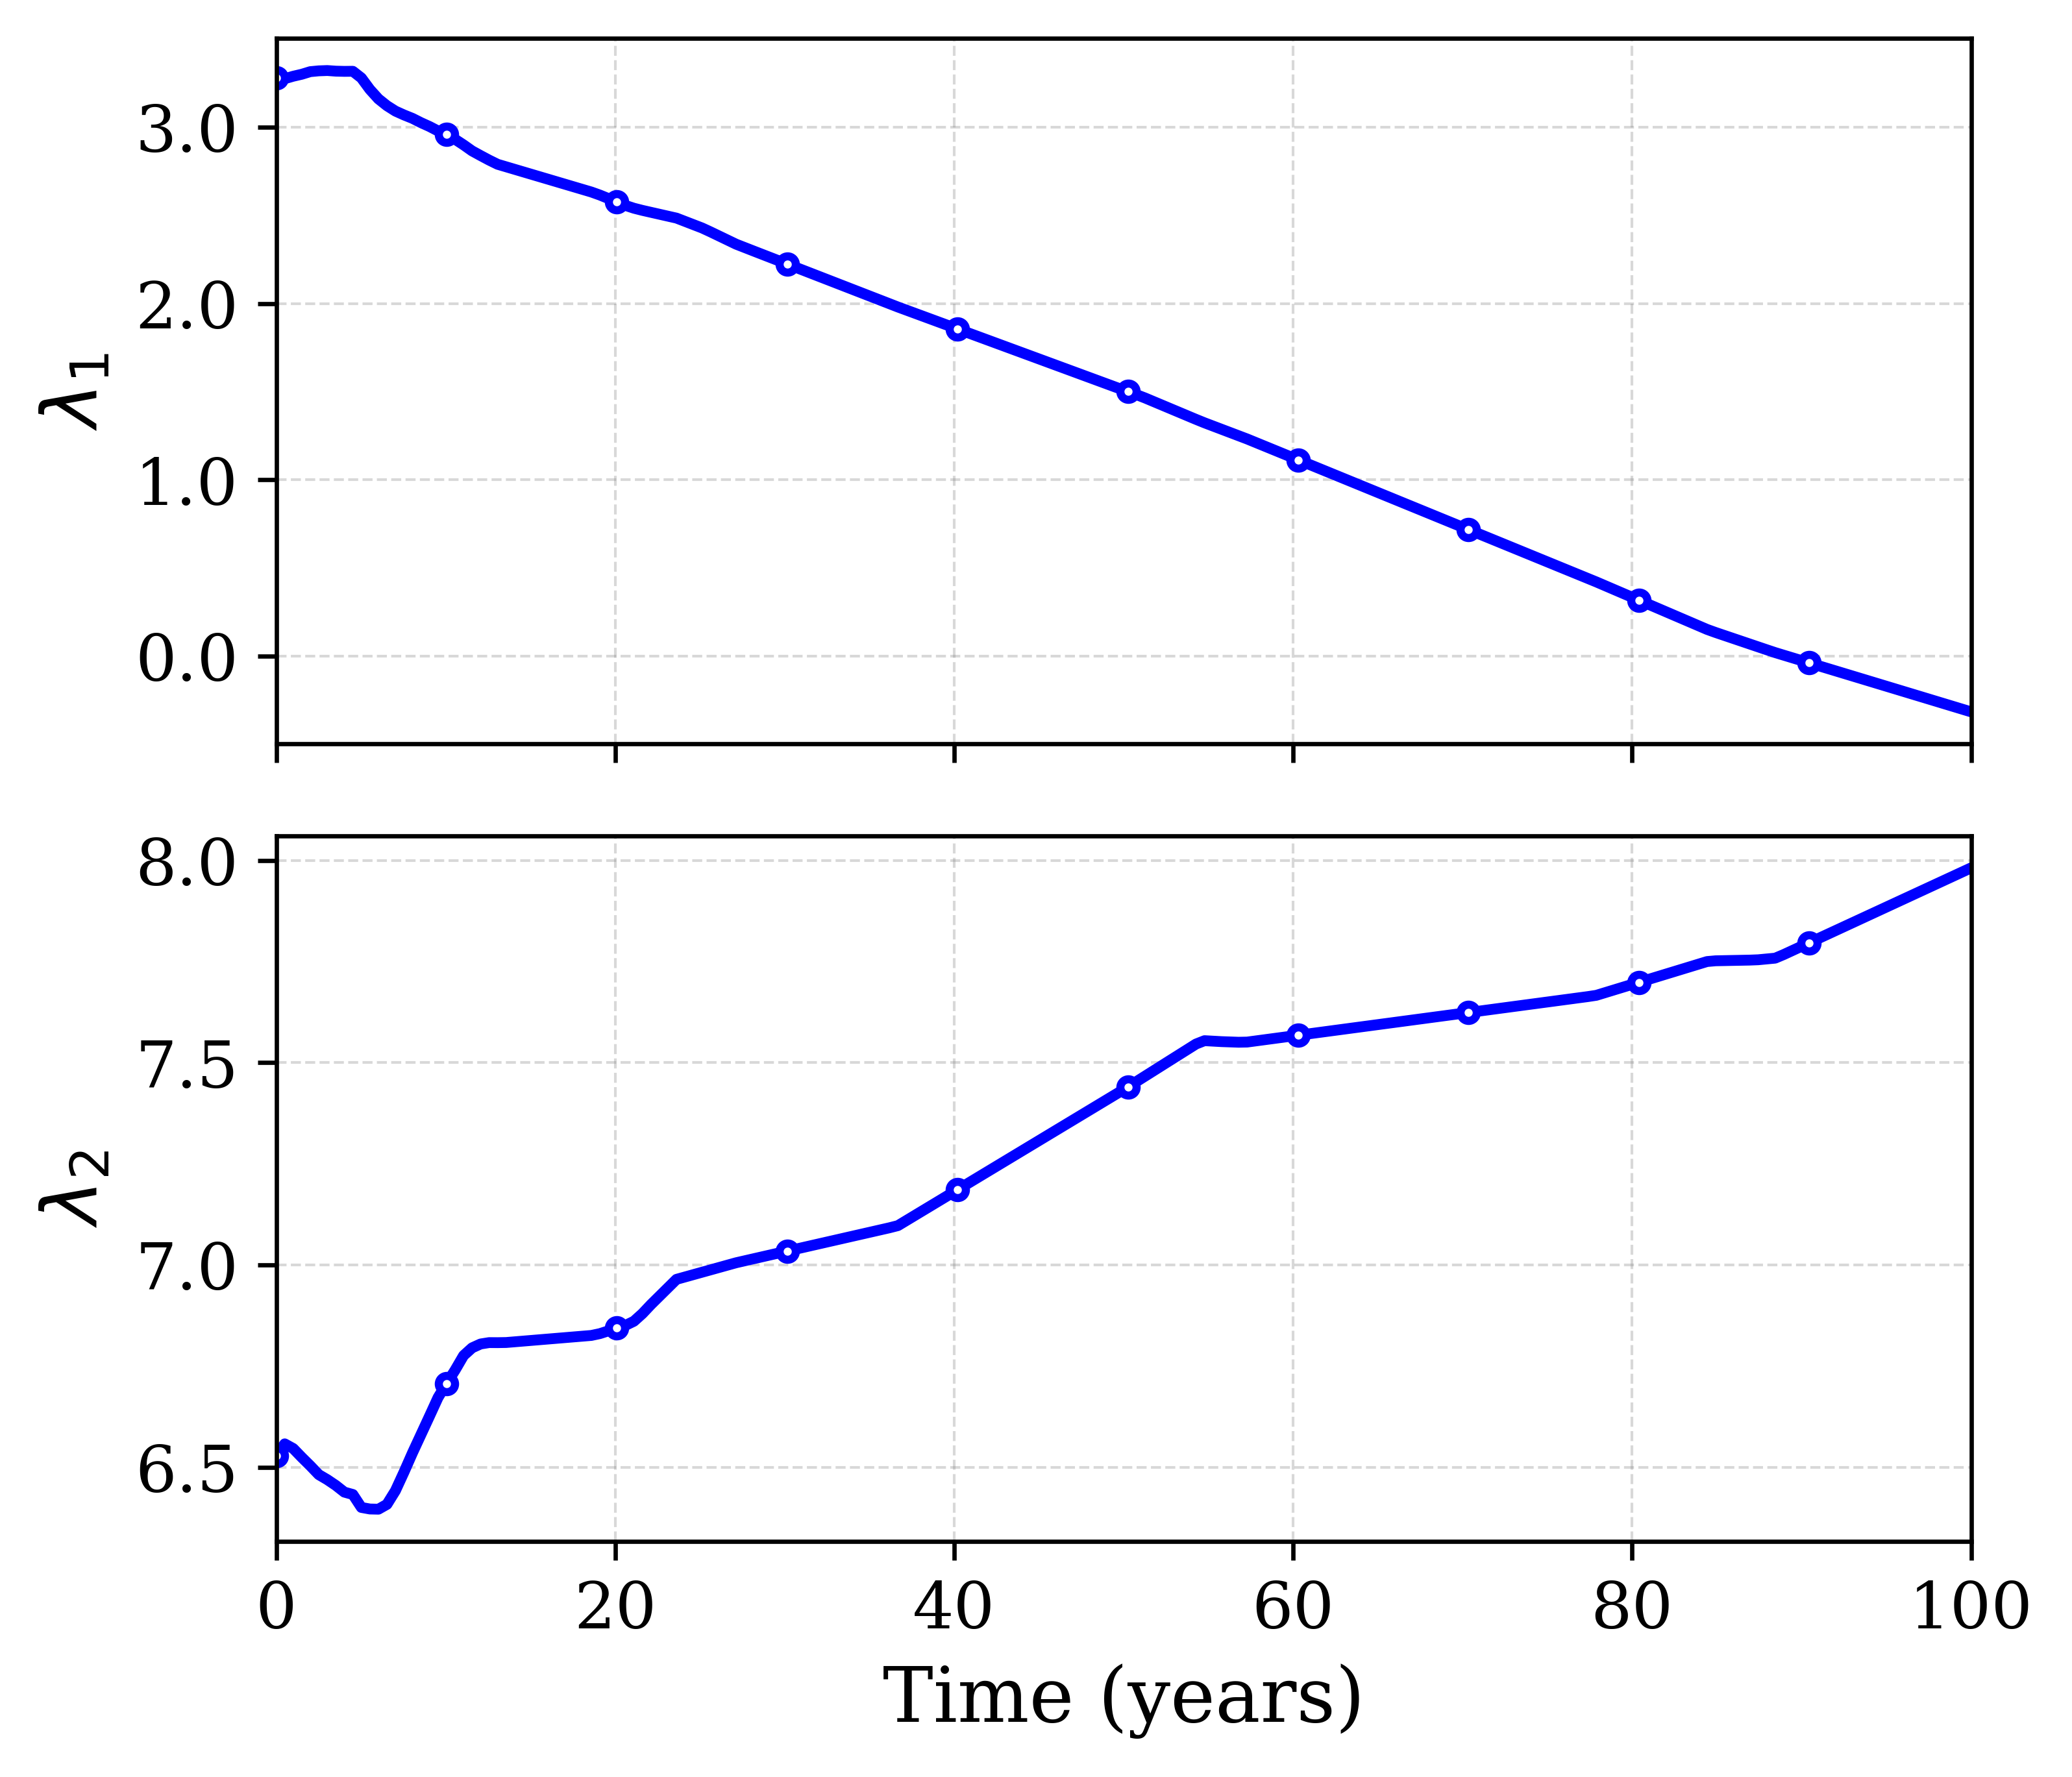
\includegraphics[width=0.75\linewidth]{z_temporal_evolution_ann_with_points_en.png}
    \caption{Temporal evolution of the GLAM parameters $\lambda_1$ and $\lambda_2$ over the service life ($t \in [0, 100]$ years) for the fixed realization $r = 5.09$ and $s = 1.80$. The continuous lines represent the ANN-based interpolation, demonstrating the model's capability to reconstruct the degradation trajectory with smoothness and consistency.}
    \label{fig:z_temporal_evolution_ann_with_points_en.pn}
\end{figure}




